%%% -*-LaTeX-*-

\chapter{Survey of Related Works}
\label{ch:related}
\section{Sampling Designs}
\label{sec:sampling}

Before analyzing any data, it must be collected either by instrumentation, experimentation, simulation, etc.
%
Under certain conditions, the input parameters may be observed rather than selected which is outside of the scope of this section.
%
Here, we formalize the different methods by which data samples can be selected for measurement/experimentation.
%
There exists two major branches on how this can be done.
%
In the first case, all of the samples are pre-selected and run in bulk.
%
We classify this type of sampling as space-filling sampling since, without any knowledge of the functional relationship, our goal is usually to spread the samples out as much as possible over the range of input values.
%
Space-filling sampling is amenable to parallelization due to the fact that the entire sample set can be specified a priori and therefore each experiment can be run independently of all other experiments.
%
Such designs attempt to capture the global behavior of the system under study and tend to focus more on uniformly sampling the entire domain of interest evenly as compared to the second mode, adaptive sampling.
%
Adaptive sampling selects the ``best'' candidate based on current information about the system.
%
The criteria for what constitutes ``best'' is investigated further in the Section~\ref{sec:adaptiveSampling}.
%
Adaptive sampling excels when only a limited region of the input domain is considered interesting or when the surrogate model is highly localized.
%
In the former case, a surrogate model can be used for extracting additional information about the data already collected, and in the latter case, the model is not expected to change significantly away from the area being sampled.
%
Adaptive sampling works in a feedback loop where new information is continuously added to a constructed model of the data which is then used to select new samples.

\subsection{Space-Filling Designs}
\label{sec:forwardSampling}

It is important to note that the methods discussed herein can be performed in the actual input space, which we will refer to as the value space, or in probability space.
%
That is, we can apply a probability distribution function (PDF) over each input, or combined inputs, and sample from the PDF rather than the input range itself.
%
In this way, we can manipulate the sampling density to favor specific regions where more fidelity may be desired or necessary, but often this requires some expert knowledge of the domain space prior to experimentation.

The two simplest forms of space-filling sampling designs are grid-based and random sampling.
%
They also represent archetypes of the two features sought after in a ``good'' space-filling sampling strategy.
%
The samples in a grid-based strategy each represent equally-sized spaces of the input domain.
%
On the other hand, they can suffer from sampling artifacts due to the regularity of sampling.
%
As an example, if a feature is aligned with the sampling grid, but occurs at a frequency greater than the grid resolution, the sampling will fail to capture the feature.
%
This type of sampling artifact is demonstrated in the left image of Figure~\ref{fig:samplingArtifacts} and leads to the problem of aliasing in signal processing~\cite{Crow1977}.
%
% A uniform grid sampling strategy also suffers from the curse of dimensionality requiring $k^d$ sammples to resolve a grid of $k$ points per dimension in $d$ dimensions.

\begin{figure}[t]
  \centering
  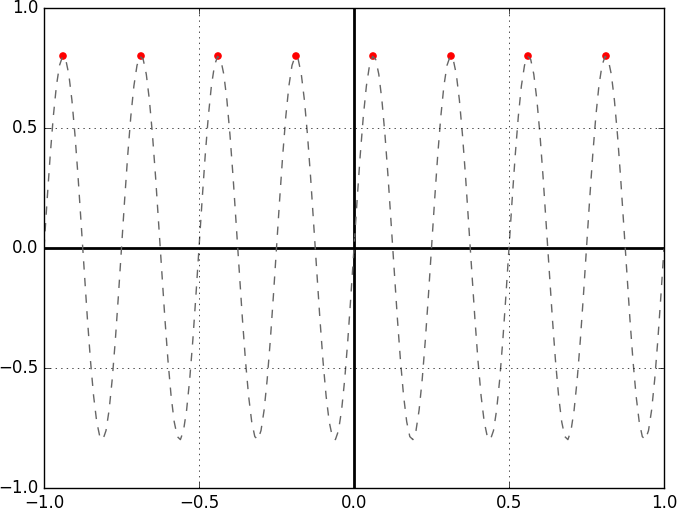
\includegraphics[width=.45\textwidth]{figs/chap3/sampledSine}\qquad
  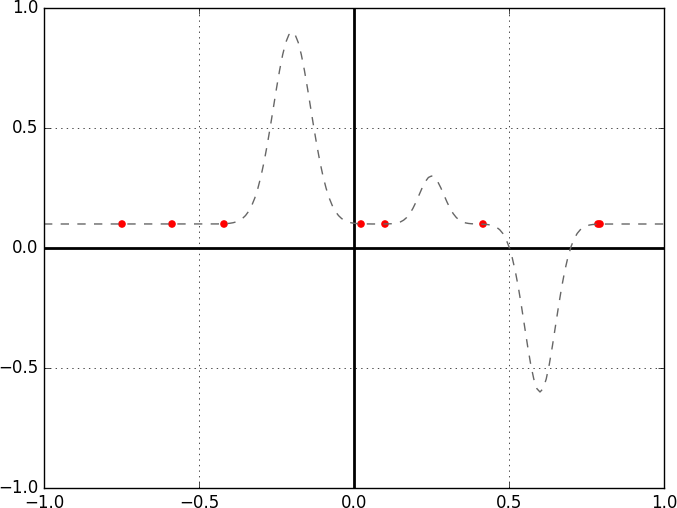
\includegraphics[width=.45\textwidth]{figs/chap3/sampledGaussian}
  \caption[1D Sampling Artifacts]{Two examples of the type of artifacts that can
  arise when performing grid sampling (left), and random sampling (right).}
  \label{fig:samplingArtifacts}
\end{figure}

On the other hand, pure random sampling counteracts this type of sampling artifact by avoiding regular patterns, but also holds no guarantees on the sampling density, thus potentially leaving large areas unsampled which could result in the sampling seen in the right image of Figure~\ref{fig:samplingArtifacts} where the variability is entirely missed.
%
Though, this may seem like a contrived example and adding more samples could alleviate this problem, even missing any one of these features could be belying crucial information to the system under study.
%
Furthermore, when moving from low to high dimensional cases, both forms of sampling suffer from the well-known \emph{curse of dimensionality}~\cite{KeoghMueen2010}.
%
In this case, as we increase the dimensionality, the volume of the space increases exponentially, thus if each sample is associated with an empty volume surrounding it (i.e., a closest point Voronoi cell~\cite{deBergCheongKreveld2008}, see description below) then the number of samples needed to maintain the same volume per sample will increase exponentially as well.
%
This means that it is intractable to cover high-dimensional spaces with ``enough'' samples if the underlying model is of a sufficiently high-frequency.
%
Thus, it is important to understand the complexity of the system under study to first determine if a global fit is feasible or desired.

Applying a probability distribution over the input space and randomly sampling the distribution function results in the very popular Monte Carlo sampling method~\cite{MetropolisUlam1949}.
%
Typically, this method has been used to estimate integrals, however it, as with all other probability-weighted sampling strategies, has the side effect of placing emphasis on a particular area of interest in the domain.
%
In this way, we minimize the likliehood that features in the particular area of interest will be undersampled.

The Latin hypercube sampling (LHS) strategy~\cite{McKayBeckmanConover1979,Tang1993,VanDam2008} attempts to bridge the gap by providing a controlled random sampling.
%
LHS divides each dimension into slabs with the condition that each slab contains only one sample.
%
Thus, in a two-dimensional setting, one can visualize this as dividing the input space into $n$ rows and $n$ columns where $n$ is the number of required samples.
%
The left two images of Figure~\ref{fig:lhsExample} demonstrate an example where $n=4$.
%
Though it does impose some structure, LHS can still suffer from the highly irregular sampling density exhibited by random sampling.
%
Again, by applying probability information we can ensure that we have higher fidelity sampling in the regions of most interest with a minimal sampling cost.
%
In this setting, the input space is divided into equally probable slabs rather than equal area.
%
Thus, if an input is sampled using a normal distribution, more cuts will be made near the mean and as we proceed away from the mean, the cuts will get farther apart and fewer samples will be required to fill these regions.

\begin{figure}[t]
  \centering
  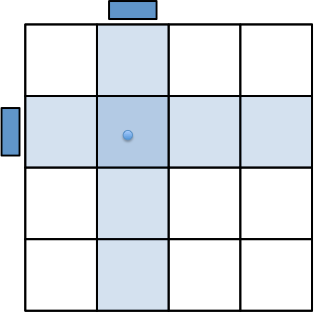
\includegraphics[width=.27\textwidth]{figs/chap3/lhs}\qquad
  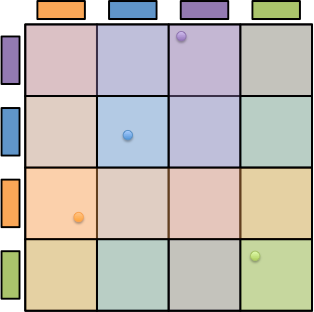
\includegraphics[width=.27\textwidth]{figs/chap3/lhs2}\qquad
  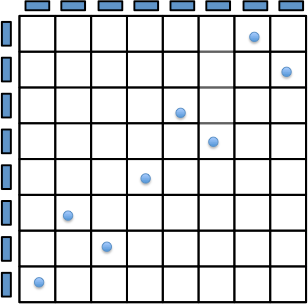
\includegraphics[width=.27\textwidth]{figs/chap3/lhs3}
  \caption[2D Latin Hypercube Sampling Example]{An example of LHS sampling in
  2D: Left: After selecting one point, we color its constituent row and column
  and prevent any more samples from being drawn from the colored cells.
  Center: The end result shows a distinct color representing each of the four
  rows and four columns. Right: An example of an undesired correlation effect appearing in an LHS design. Such an correlation can be mitigated with the use of appropriate techniques.}
  \label{fig:lhsExample}
\end{figure}

LHS designs can also produce random correlations in the sampling, as can be seen in the right image of Figure~\ref{fig:lhsExample}.
%
To this end, the permutation matrix used to construct the LHS sample can be manipulated to reduce such correlation effects when the number of samples is greater than the dimensionality~\cite{ImanConover1982,Owen1994}.
%
These correlation reducing strategies however may introduce bias~\cite{OlssonSandbergDahlblom2003}.

In computer graphics, practitioners often use blue-noise distributions of samples which have been found to match the arrangement of photoreceptors in our eyes~\cite{Yellott1982}.
%
The term blue-noise comes from signal processing and relates to the power spectrum of the noise signal~\cite{Tuzlukov2002}, but also equally applies with respect to density in the spatial domain.
%
Blue noise exhibits no concentrated spikes (i.e., small area with many samples, respective to the rest of the domain) and minimal low frequency components (i.e., large area with few samples, respective to the rest of the domain)~\cite{YanGuoWang2015}.
%
In a geometric sense, the sample points will exhibit no regularity, but will still be uniformly distributed in the domain space.
%
The main techniques for achieving a blue-noise sampling include Poisson disk sampling, relaxation methods, and tile-based methods~\cite{YanGuoWang2015}.

The first method, Poisson disk sampling creates samples that are guaranteed to be a minimum distance from all other samples and is used widely in computer graphics.
%
The classic algorithm applies to the two dimensional case and is achieved through rejection sampling, that is points are iteratively added to the overall sample set if they do not lie inside a disk of specified radius~\cite{Cook1986}.
%
Accelerations off of this baseline algorithm focus on methods for efficiently tracking the empty regions left to be sampled in order to reduce the likliehood of rejecting future samples~\cite{EbeidaDavidsonPatney2011,EbeidaMitchellPatney2012,GamitoMaddock2009,Jones2006,JonesKarger2011,WhiteClineEgbert2007}.
%
Though most graphics problems deal in relatively low dimensional spaces, there has been some recent work for computing Poisson disk sampling in arbitrary dimensions~\cite{Bridson2007,EbeidaMitchellPatney2012,EbeidaMitchellPatney2015,GamitoMaddock2009,MitchellEbeidaAwad2018} and with the correct application of acceleration structures such as a kd-tree, these methods are viable up to tens of dimensions~\cite{MitchellEbeidaAwad2018}.

Of the relaxation techniques, Centroidal Voronoi tessellation (CVT)~\cite{DuFaberGunzburger1999} has been the most widely studied.
%
CVT is related to $k$-means clustering~\cite{HastieTibshiraniFriedman2008} in terms of computation and can be employed to provide a sampling strategy that provides uniform sampling density without being aligned to a particular grid.
%
The idea is based on the closest point Voronoi diagram~\cite{deBergCheongKreveld2008}.
%
Given a set of \emph{sites} existing in $\mathbb{R}^d$, the closest point Voronoi diagram decomposes the space such that any location is associated to its closest representative \emph{site} under some distance metric, typically Euclidean.
%
CVT works by aligning the center of mass, or centroid, of each Voronoi cell with its \emph{site} which then becomes the sample point.
%
By aligning the centroid to the Voronoi cells, we create a solution whereby each Voronoi cell is of roughly equal size (excluding cells on the boundary which extend to infinity), or in other words, the samples are equidistant or nearly equidistant from one another.
%
Naive CVT can suffer from regularity as patterns can exist in the resulting sample set.
%
To this end, several optimizations have been performed to improve the blue noise characteristic~\cite{BalzerSchlomerDeussen2009,ChenYuanChoi2012,deGoesBreedenOstromoukhov2012,XuLiuGotsman2011}.
%
As with Poisson disk sampling, most research has been focused on the low-dimensional setting since the combinatorics of increasing dimensionality incur a large storage overhead when processing the Voronoi diagram in arbitrary dimension~\cite{BoissonnatChazalYvinec2017}.
%
However, Lloyd's method~\cite{DuFaberGunzburger1999} can be used to iterate to an approximate solution for moderate dimensionality which we utilize in Chapter~\ref{ch:graphs} for the construction of cone graphs using a constrained CVT.

Lastly, tile-based methods create small, repeatable templates which can be repeated over the domain of interest~\cite{HillerDeussenKeller2001,KopfCohenOrDeussen2006,LagaeDutre2005,Ostromoukhov2007,OstromoukhovDonohueJodoin2004,WachtelPilleboueCoeurjolly2014}.
%
In this setting, a small patch or tile of the domain is pre-computed with desired blue-noise characteristic.
%
If the boundaries are carefully constructed to be periodic or otherwise aligned in some fashion, then the tiles can be combined to create a larger domain that maintains the blue-noise property.
%
One can see that as the dimensionality increases, so do the boundaries that need to be matched and so most of these methods are applied to two-dimensional domains.

Another class of space-filling designs that have existed for a long time are quasi-random or low-discrepancy sequences which have been used a lot for quasi Monte Carlo methods in numerical analysis~\cite{Niederreiter1992}.
%
The low discrepancy paradigm is similar in spirit to the category of blue-noise sampling, but using a different mathematical definition based on \textit{discrepancy} of points which basically is a measure of how much a sequence deviates from an ideal equally distributed sequence.
%
One drawback is that these methods are deterministic and can result in repeating patterns which could suffer from the aliasing artifact highlighted in Figure~\ref{fig:samplingArtifacts}.
%
Examples include the one-dimensional Van der Corput sequence~\cite{vanderCorput1935}, its higher dimensional generalization known as the Halton sequence~\cite{Halton1964,BraatenWeller1979}, the Hammersley set~\cite{HammersleyHandscomb1964}, and the Sobol sequence~\cite{Sobol1967}.

\subsection{Adaptive Designs}
\label{sec:adaptiveSampling}

In contrast to the techniques described above, adaptive sampling selects new candidate samples by utilizing all of the previously collected information, and therefore, the full set of samples cannot be generated a priori.
%
Another term commonly used in the data mining community is active learning and spans a wider class of algorithms aimed more broadly at the problems of classification and regression~\cite{Settles2009}.
%
Other names appear in the literature as well such as sequential sampling and optimal experimental design.
%
We focus our attention specifically on the problem of regression over real-valued domains, and follow the general adaptive sampling pipeline laid out in Figure~\ref{fig:asCycle} which is repeated until a convergence criterion is met, typically the residual between consecutive iterations falls below a preset threshold.

\begin{figure}[t]
  \centering
  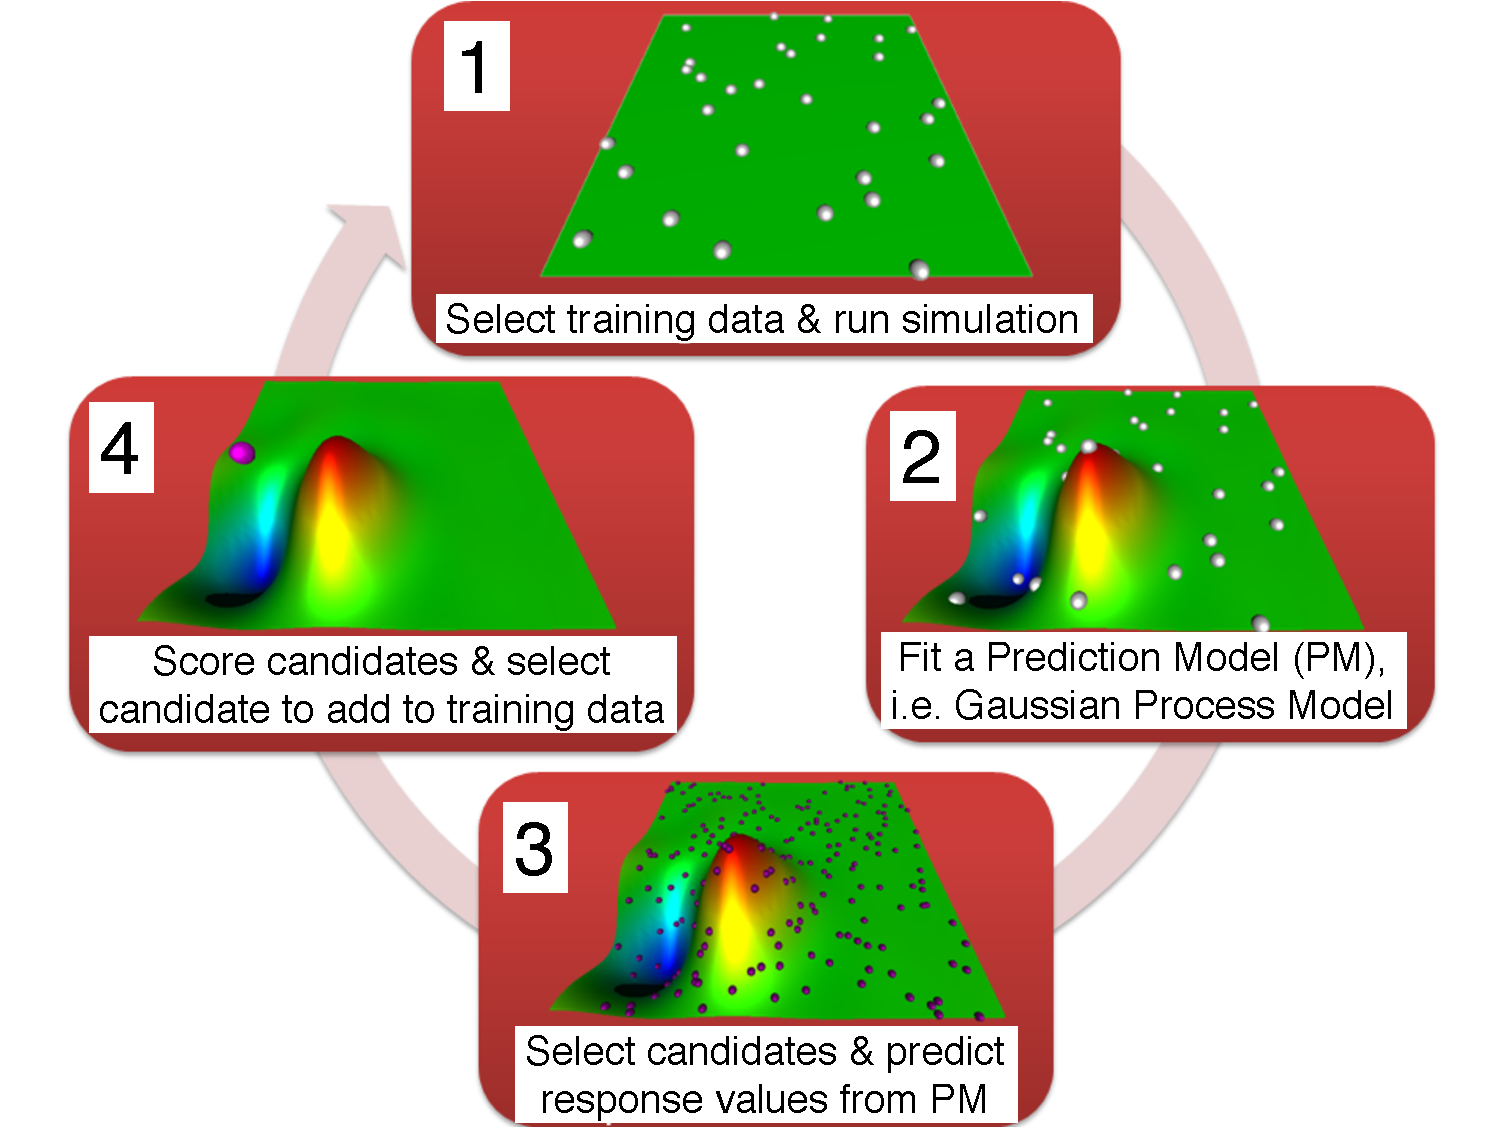
\includegraphics[width=.75\textwidth]{figs/chap3/pipeline}
  \caption[Adaptive Sampling Cycle]{A broad picture of the adaptive sampling
  cycle.}
  \label{fig:asCycle}
\end{figure}

The cycle begins by querying the oracle or ground truth model using an initial sampling of the input space, such as a sparse version of one of the space-filling designs presented in Section~\ref{sec:forwardSampling}.
%
With the queried information, we then build a predictive model of the system.
%
% Various types of predictive models are reviewed in Section~\ref{sec:regression}.
%
The predictive model allows us to score or rank the input space or a sample set derived from it.
%
From the scored candidates, one or more points is/are selected to be sent to the oracle for querying.
%
The new information is added to the predictive model and the cycle repeats until the specified convergence criterion is met.

Variations of this theme have been explored at every stage in the cycle.
%
As discussed in Section~\ref{sec:forwardSampling}, various initial sampling designs can be employed for building an initial model.
%
In Section~\ref{sec:regression}, we will look at various types of predictive models.
%
In this section, we focus on the selection and scoring of candidate points under different settings.
%
We pay specific attention to adaptive sampling in the context of global surface fitting, limit surface refinement, and batch selection where more than one point is selected before retraining the predictive model.
%
Afterwards, we review the related works within the visualization community in an area known as design steering where the adaptive process includes human involvement rather than being completely automated.

\subsubsection{Global Fitting Problems}

Adaptive sampling has been used to train neural networks, Gaussian mixture models, and locally weighted regression models among others~\cite{CohnGhahramaniJordan1996}.
%
Most of the methods described herein can be accomplished by employing a scoring function upon which all of the candidates can be evaluated and ranked.
%
The basic process of global adaptive sampling tries to converge to an acceptable fitting of a surrogate model using fewer data points than the more standard space-filling designs described in Section~\ref{sec:forwardSampling}.
%
Techniques for achieving this include reducing global uncertainty~\cite{CohnGhahramaniJordan1996,TongKoller2001}, exploiting areas of high gradient~\cite{MaljovecWangKupresanin2013}, and focusing on otherwise ``interesting'' regions.
%
Interesting in this context can mean several different things such as unexplored regions~\cite{Whitehead1991}, regions of low confidence~\cite{ThrunMoller1992}, poorly fit regions~\cite{LindenWeber1993}, areas of expected change~\cite{CohnAtlasLadner1990,CohnAtlasLadner1994}, and/or areas where information gain is optimal~\cite{Lam2008}.
%Maybe we should dig into each of these a bit more thoroughly? Like what are the drawbacks of each, or why is directly extracting the topology well-aligned with what some of these are already attempting to accomplish.

A slightly modified version is aimed at global optimization rather than global accuracy of the model~\cite{MooreSchneider1996,JonesSchonlauWelch1998}.
%
In this context, the goal is to identify a global optimal parameter setting where either a single figure of merit is maximized or minimized or a Pareto optimum that trades off amongst several figures of merit is optimized.
%
The active search method takes a slightly different approach by looking at the problem as attempting to sample points contained in a single class~\cite{GarnettKrishnamurthyXiong2012}.
%
This last case is related to the problem of limit surface recovery discussed below in Section~\ref{sec:limitSurface} where we are interested in defining the boundary between two classes.

Most of these methods exploit geometric or statistical properties of the data, but none have explored the topological impact of the data as proposed in this body of work (See Chapter~\ref{ch:adaptiveSampling} for more details).

\subsubsection{Limit Surface Problems}
\label{sec:limitSurface}

On the border between regression and classification is the notion of thresholding.
%
That is, when learning a regression model, the user is less interested in the value of the response surface, but more in its ability to detect when the response lies above or below a particular threshold value.
%
This is a common problem in risk assessment where the isocontour specified by the threshold value is called the limit surface and it separates the success region from the failure region.
%
Engineers are often concerned with identifying such limit surfaces and characterizing them in order to perform trade-off analysis and to set adequate safety margins.
%
The problem is different from global fitting in that the overall fidelity is less of a concern as long as the behavior is adequately modeled around the limit surface.
%
This problem of limit surface identification is similar to what is called decision boundary analysis in the classification problem setting~\cite{DiamantiniPotena2007,GoLee2003,LeeLandgrebe1993,LeeLandgrebe1997,WooLee2017,ZhangLiu2005}.
%
However, it also differs from classification (i.e., discrete labeling which typically results in a binary decision of inside or outside a particular class) since knowing the gradient direction and magnitude along and near the limit surface can also be useful information.

In reliability engineering, this problem is known as determining the limit state function and can be thought of as the point where a system's load exceeds its capacity where load and capacity are functions of the input parameters.
%
The literature in this field attempts to either converge to a single most probable point (MPP) through nonlinear optimization methods~\cite{EldredBichon2006,EldredAgarwalPerez2007} or through adaptive sampling~\cite{Wu1994,DeyMahadevan1998,ZouMahadevanMourelatos2002,BichonEldredSwiler2008}.

In the statistics literature, Ranjan et al.~\cite{RanjanBinghamMichailidis2008} have attempted to solve this problem by defining an expected improvement candidate scoring function that harnesses both a prediction's proximity to the threshold value and also the uncertainty associated with the prediction.
%
In similar spirit, the machine learning community has designed similar yet simpler scoring functions that take advantage of similar information.
%
Bryan et al.~\cite{BryanSchneiderNichol2005} define a scoring function called the straddle function, and Gotovis et al.~\cite{GotovosCasatiHitz2013} introduce the ambiguity scoring function which can be thought of as a generalized version of the straddle function.
%
All three methods utilize a Gaussian process surrogate model, however the latter two are performed in what Settles~\cite{Settles2009} refers to as the pool-based active learning setting, whereas the first uses a global optimization to select the optimal point at each iteration which drastically increases the overhead per iteration.

% \subsubsection{Optimization Problems}
\subsubsection{Design Steering}
\label{sec:designSteering}

The aforementioned methods are assumed to be completely automatic except in the instance where the human is required to act as the oracle, though such settings are more rare in the regression (i.e., continuous) context than in the classification (i.e., discrete) context.
%
%The latter context of classification is beyond the scope of this work.
%
% For example, a common human-dependent task more often involves annotating data with text labels rather than assigning often subjective numeric ranks or values to items in a dataset.
%
Within the visualization community, several works have explored the notion of design steering where the results require either a qualitative examination or are used to inform indirect decisions rather than in a direct sampling feedback loop.

HyperMoVal~\cite{PiringerBergerKrasser2010} is a software system used for validating regression models against actual data.
%
It uses support vector regression (SVR)~\cite{SmolaScholkopf2004} to fit a model to high-dimensional data, highlights discrepancies between the data and the model, and computes sensitivity information on the model.
%
The software allows for adding more model parameters to refine the regression to an acceptable level of accuracy.
%
Berger et al.~\cite{BergerPiringerFilzmoser2011} utilize two different types of regression models (SVR and nearest neighbor regression) to analyze a trade-off study in performance car engine design.
%
Utilizing the predictive power of the regression, they are able to provide a guided navigation of the high-dimensional space centered around a user-selected focal point.
%
The user adjusts the focal point through multiple linked views, and sensitivity and uncertainty information are encoded around the focal point.

Tuner~\cite{Torsney-WeirSaadMoller2011} employs an automated adaptive sampling algorithm where a sparse sampling of the parameter space is refined by building a Gaussian Process Model (GPM)~\cite{RasmussenWilliams2006}.
%
The adaptive sampling focuses additional samples in areas where either the response is near an optimal setting or the model has high uncertainty.
%
The software then relies heavily on user interaction to study the sensitivities with respect to each input parameter and steers the computation toward the user-defined optimal solution.
%
Demir et al.~\cite{DemirWestermann2013} improve the effectiveness of GPMs by utilizing a block-wise matrix inversion scheme that can be implemented on the GPU, greatly increasing efficiency.
%
In addition, their method involves progressive refinement of the GPM and can be halted at any point, if the improvement becomes insignificant.

Most of these methods convey sensitivity information through user exploration of the input space.
%
We discuss sensitivity in more detail in Section~\ref{sec:sensitivity} and in Section~\ref{sec:SA_visualization}, explicit visual encodings for understanding sensitivity information are also discussed.
%
Sensitivity analysis plays a major role in the novel system described in Chapter~\ref{ch:visualization}.

\section{Proximity Graphs}
\label{sec:graphs}

Our target datasets are presented as point sampled data of low to moderate ($<$100) dimensionality.
%
Many common analysis techniques on such data require the imposition of some structure to relate the disjoint set of point samples.
%
Such a structure could be used to interpolate, cluster, filter, or project/warp the data.
%
Depending on several factors including: the questions being asked, the dimensionality of the data, and the distribution of the point samples, the correct choice of structure among the points could vary.
%
For example, in low dimensional settings, it is often common to polygonize or triangulate point-sampled data, but the combinatorics of representing the high-dimensional equivalents of surfaces and volumes of even a simplicial complex quickly become infeasible to store and operate on.
%
What is more often found in higher dimensional settings is the use of 1-skeleton structures such as those given by proximity graphs.
%
Proximity graphs connect nearby points in a point set via a set of edges where the presence of an edge is based on different geometric constraints depending on the choice of graph.

The proximity graphs we consider fall into one of three families: distance-based, empty region, and cone-based.
%
The distance-based graphs include the $k$-nearest neighbor graph and $\epsilon$-ball graph.
%
The empty region graphs include the Delaunay graph, the diamond graph, the Gabriel graph, the relative neighbor graph, and the remaining family of $\beta$-skeletons.
%
Cone-based graphs include Yao graphs and the semi-Yao or $\Theta$-graphs.
%
Such 1-skeleton graphs can be prone to over- and/or under-connect a point cloud depending on how the data is distributed.
%
Both over- and under-connected graphs can result in misleading data representations.
%
Though efforts have been made to improve the neighborhood quality in high dimension, these issues can still not be wholly avoided.
%
In other words, there is no silver bullet.
%
Since properties of these various graphs vary drastically, it is important to understand the implications of using a particular graph or the alternatives that may exist.

\subsection{Distance-Based Graphs}
Distance-based graphs are by far the most widely used and well-studied of the three families of graphs named in the introduction.
%
In fact, the methodology we propose begins with an efficient approximate $k$-nearest neighbor graph in order to prune other graphs from it.
%
The two main distance-based graphs are the $k$-nearest neighbor ($k$-nn) graph and the $\epsilon$-nearest neighbor ($\epsilon$-nn) graph.
%
The sphere of influence graph~\cite{Toussaint1988} can also be considered in this family of graphs, though it is much less commonly used and also belongs to a family of graphs known as intersection graphs which we do not consider as relevant to this body of work.

A $k$-nearest neighbor graph, in our setting, is an undirected graph where an edge exists between two points, $p$ and $q$, if $q$ is one of the $k$ closest points to $p$ or vice versa in some defined metric space.
%
The related $\epsilon$-nearest neighbor, also known as the $\epsilon$-ball graph or fixed radius graph, instead is an undirected graph where an edge exists between $p$ and $q$ if the distance metric is less than a specified $\epsilon$.
%
Both of these settings give a somewhat incomplete, but complementary view of the data.
%
On one-hand, $\epsilon$-nn graphs will use more edges to connect points in a more densely-packed region of space.
%
On the other hand, $k$-nn graphs will guarantee every point is connected to at least $k$ other points which is useful for connecting outliers or sparsely sampled regions to the rest of the data.
%
We choose to focus our study on the $k$-nearest neighbor graph due to our ability to more sensibly tune the $k$ parameter and its prevalence in the literature.

There exist several state of the art competing libraries for computing both exact and approximate $k$-nearest neighbor graphs.
%
The methodologies use data structures such as space-partitioning trees~\cite{Bentley1975,LiuMooreGray2004,Omohundro1989,Uhlmann1991,Yianilos1993}, product quantization~\cite{BabenkoLempitsky2012,JegouDouzeSchmid2011} locality-aware hashing~\cite{BawaCondieGanesan2005,LvJosephsonWang2007,AndoniIndyk2008,TsaiYang2014,ZhaoLuMei2014}, pemutation indices~\cite{Esuli2012,TellezChavezNavarro2013}, and graphs~\cite{AryaMount1993,DongMosesLi2011,HouleSakuma2005,IwasakiMiyazaki2018,MalkovYashunin2018,SebastianKimia2002,WangLi2012} in order to perform fast proximity queries.
%
These methodologies vary in their ability to represent the exact versus approximate solutions.
%
For the purposes of our later studies, we consider the approximation quality of all methods ``good enough.''
%
This is due to the fact that when using such an approximate knn throughout this document, we will be extracting many more neighbors than required in order to prune this graph using one of the remaining techniques.
%
In cases, where we compare or use knn in isolation, we select an exact $k$-nn for comparison.
%
Recently, Johnson et al. have demonstrated how to effectively perform exact $k$-nn search on the GPU, thus offering the fastest known exact $k$-nn implementation to date with the FAISS library which also supports GPU computation of approximate $k$-nn searches~\cite{JohnsonDouzeJegou2017}.
%
For evaluating efficiency of the various approximation algorithms, consider the benchmarks developed by Aumuller et al.~\cite{AumullerBernhardssonFaithfull2017} and Chisholm et al.~\cite{ChisholmRichmondMaddock2016}.

\subsection{Empty Region Graphs}
Consider two points $a$ and $b$ are elements of a $d$-dimensional point set, $a,b \in P \subseteq \mathbb{R}^d$.
%
In the empty region graph setting, an edge exists between $a$ and $b$ if and only if there exists a region, $R(a,b) \subseteq \mathbb{R}^d$, that does not contain any other point in $P$, $R(a,b) \cap P = \emptyset$.
%
Depending on the definition of $R$, different graphs can arise.
%
Noteworthy, examples include the relative neighbor graph~\cite{Toussaint1980}, its approximation the Urquhart graph~\cite{Urquhart1980}, and the Gabriel graph~\cite{GabrielSokal1969} which are examples of a class of graphs known as $\beta$-skeletons~\cite{KirkpatrickRadke1985,JaromczykToussaint1992}.
%
It is worth noting, that two definitions of the $\beta$-skeleton exist, namely the \emph{circle-based} and the \emph{lune-based} approaches.
%
We will be referencing the \emph{lune-based} definition given in Section~\ref{sec:bpskeleton} unless otherwise noted.

The $\gamma$-neighborhood is an attempt to unify the 2D circle-based $\beta$-skeletons, Delaunay triangulation, and convex hull of a point set into a two-parameter family of techniques~\cite{Veltkamp1991}.
%
Other examples of graphs in this family include the diamond graph~\cite{CorreaLindstrom2011}, the Delaunay graph (where the empty region is defined over $d-1$ points)~\cite{Delaunay1934}, the $\sigma$-local graph (where the empty region is two disjoint components centered at each of the endpoints)~\cite{BoseColletteLangerman2010}, and infinite strip graphs~\cite{Veltkamp1991,CardinalColletteLangerman2009}.
%
Similar to the generalization of the Gabriel graph and relative neighbor graph into the $\beta$-skeleton~\cite{KirkpatrickRadke1985} or Veltkamp's approach with the $\gamma$-neighborhoods, in Chapter~\ref{ch:graphs}, we develop the $\beta_p$-skeleton which unifies the entire family of lune-based $\beta$-skeletons with the canonical diamond graph used by Correa and Lindstrom and the infinite strip graphs into a two-parameter $(\beta,p)$ family of graphs that also includes a spectrum of graphs occuring between these examples.

Kowaluk et al.~\cite{JaromczykKowaluk1987,KowalukMajewska2014} have studied relative neighbor graphs and $\beta$-skeletons under various $L^p$-spaces which is different than our regime of using $p$-norms as generators for shapes to be evaluated in $L^2$-space.
%
Note, the shapes we use for empty regions will always be both radially symmetric about the edge and also symmetric about the perpendicular bisector of the edge.
%
This condition does not hold for the cases defined by Kowaluk et al.
%
Furthermore, under discretization (see Section~\ref{sec:gpu_bp_discrete}), we are able to generalize our method further to utilize any 1D function as a generator for a symmetric, high-dimensional shape to be used as an empty region.

Lastly, $\gamma$-visibility graphs~\cite{KatzTalBasri2007,KatzTal2015,KatzTal2017} are another means of generalizing $\beta$ skeletons to include not only non-uniform shapes, but non-symmetric shapes.
%
In some ways this technique allows for more generic shapes than our own which is restricted to radially symmetric shapes, but as noted by the authors, the work is largely theoretical and we instead focus on an intuitive shape parameterization that generalizes well to higher dimensions.

\subsection{Cone-Based Graphs}
\label{sec:bg_cones}

Cone-based graphs are so-called because they carve the space around a specific point $a$ into equal-sized cones and draw a fixed sample size from each conic section to connect to $a$.
%
These graphs are of interest to us because they are similar in spirit to the notion of the space-pruning umbras defined by Correa and Lindstrom~\cite{CorreaLindstrom2011}.
%
However, splitting high-dimensional spaces into equal-sized hypercones is a challenge that we attempt to approximate using clever sampling.

The methods within this class differ in how points are selected from each conic section.
%
The Yao graph selects the closest point in each conic section to be a neighbor of $a$~\cite{Yao1982}.
%
The $\Theta$-graph, or semi-Yao graph, selects the point whose projected distance from the point onto the cone's axis is closest as a neighbor of $a$~\cite{Clarkson1987,Keil1988}.
%
Rahmati et. al generalized this graph to connect $a$ to $k$ neighbors in each section and called it the $k$-semi-Yao graph~\cite{RahmatiKingWhitesides2013}.
%
We consider this generalization for both Yao and $\Theta$-graphs and call them $k$-Yao and $k$-$\Theta$ graphs for simplicity.

\section{Sensitivity Analysis}
\label{sec:sensitivity}

Sensitivity analysis (SA) studies how changes in the model inputs affect the outputs and can take many different mathematical forms.
%
Broadly speaking, SA methods can be categorized as being local, relative to point estimates of the parameter space, or global which considers the entire parameter distribution~\cite{Hamby1995}.
%
Local SA or differential SA studies the change of model response around specific locations in the input space and is often useful for doing deep analysis on a subset of a larger corpus of data.
%
One example may be to understand the behavior around several local optima of a model to determine the most ``stable'' feature of the data.
%
Another example might be to understand the behavior around an outlier or anomaly in the data generated from the model.
%
Global sensitvity methods, on the other hand, are able to rank the overall importance of each model input and in some cases identify redundant features.
%
As such, an application for global sensitivity analysis can be dimensionality reduction where the goal is to reveal important subspaces of the original problem.
%
These subspaces can help us avoid the \emph{curse of dimensionality} allowing us to sample the subspace more robustly and compute subsequent analysis more efficiently.

\subsection{Local Sensitivity Analysis}

Differential SA computes the location-dependent partial derivatives of the output(s) with respect to each input parameter as can be seen in methods such as brute force finite differencing using a surrogate model when neighboring data is not readily available.
%
That is, take a small step along one axis and evaluating the slope between the perturbed point and the reference point and repeating for each dimension.
%
Improvements to the finite differencing scheme exist that are less computationally expensive such as the decoupled direct method~\cite{Dunker1981,Dunker1984} which solves the problem as a sytem of ordinary differential equations and the Green function method~\cite{KramerCaloRabitz1981} which can be faster when the ratio of inputs to outputs is very high, but is more complicated and thus prone to higher numerical errors~\cite{SaltelliChanScott2000}.

\subsection{Global Sensitivity Analysis}

Common global sensitivity methods include regression analysis, correlation analysis, screening methods, and variance-based techniques.
%
Regression analysis~\cite{Galton1886} is one of the oldest methods used today.
%
The process works by fitting the data with a linear model and reporting the solved linear coefficients as the standard regression coefficients (SRCs).

Correlation analysis represents another class of methods that are fairly simple to implement and understand.
%
Correlation analysis uses the covariance of two variables (typically one input and one output) in order to describe the significance of their functional relationship.
%
Such methods include the Pearson correlation coefficients~\cite{Pearson1895} which measure the linearity between two parameters.
%
The slightly more robust Spearman rank correlation coefficients~\cite{Spearman1904a} and Kendall rank coefficients~\cite{KendallGibbons1990} measure the monotonicity between parameters and can thus capture nonlinear, but still monotonic, relationships.

Screening methods measure the amount of information gained/lost when one or more inputs are removed from a parametric model or allowed to vary.
%
Such methods include the simple Morris one-at-a-time (MOAT)~\cite{Morris1991} which repeatedly computes the local SA and collects the information into a statistical average and standard deviation for each input.
%
More complicated versions, employ complex surrogate models and determine sensitivities from the hyperparameter settings.
%
These include multivariate adaptive regression spline (MARS) screening~\cite{Friedman1991} and Gaussian Process screening~\cite{RasmussenWilliams2006}.

The more powerful variance-based methods include such techniques as Sobol sensitivity indices~\cite{Sobol1993} and Fourier amplitude sensitivity testing (FAST)~\cite{CukierFortuinShuler1973} which are able to capture higher order sensitivities that the preceding methods do not.
%
The tradeoff here is these methods are more complicated to compute.

The global methods discussed thus far do not directly reduce the dimensionality, but instead associate values that can be considered as ranks or scores to each input parameter.
%
From this ranking, the user can either directly select the number of parameters to include in any reduced anaylsis, or the number of parameters can be computed given a specified error threshold.
%
The remaining methods instead attempt to reduce the dimensionality by transforming the model input space to be a linear combination of the original model inputs.
%

\subsection{Dimensionality Reduction Methods for Sensitivity Analysis}

Recall that one main goal of understanding sensitivity is to reduce the problem space into a more tractable or human-comprehensible domain without sacrificing much in the way of model fidelity.
%
It turns out there are a class of methods directly designed for this purpose, although not all of them respect the functional relationship between input parameters and output responses.
%
Broadly speaking, such dimensionality reduction methods can be classified into two categories: linear and non-linear methods.
%
I will briefly review them here.

\subsubsection{Linear Dimensionality Reduction Methods}

Linear dimensionality are so-called because they seek to find a single linear projection operator that can be applied to the data that best preserves some quality of the data.
%
The methods differ in the quality of the data that they attempt to maintain.
%
This linear projection operator can be expressed as an $M \times N$ matrix where $N$ is the original dimensionality of the problem and $M$ is the size of the reduced space.
%
Within the visualization community, we often set $M$ to two or three so we can directly visualize the results.

From a sensitivity analysis standpoint, the reduced dataset is less interesting to us than the transformation matrix.
%
Each column of the transformation matrix tells us how much weight a particular input parameter has in the reduced space.
%
For example, a column of small magnitude (relative to the rest of the matrix) or zero values tell us that the corresponding original input parameter represents redundant information that is less useful in identifying distinct data points when compared to the expressive power of the other input parameters.
%
Looking at it another way, the rows of the transformation matrix tell us which original input parameters are combined in order to construct one dimension of the lower dimensional space.
%
For a comprehensive survey of linear dimensionality techniques, I defer to the excellent work of Cunningham and Ghahramani~\cite{CunninghamGhahramani2015}.
%
I will instead review the most widely adopted methods and their relevant extensions.
%
This will give us enough information so as to understand the advantages and disadvantages of linear dimensionality reduction as a tool for understanding sensistivity.

Principal Component Analysis (PCA) is a common technique that can be described in two different ways.
%
The first formulates the dimensionality reduction problem as minimizing the sum of squared residuals between projected data points and their original counterparts~\cite{Pearson1901}.
%
Equivalently, PCA maximizes the variance of the data in the lower dimensional space~\cite{Hotelling1933}.
%
Several extensions have been made to the classical PCA solution framing the problem in unique settings such as a probabilistic model, kernel feature space, robustness to outliers, sparse solutions, and nonlinear solutions.

Note, that not all of these variants are applicable for sensitivity analysis and some seek to solve different goals.
%
For instance, kernel PCA first projects the original data into a feature space using a kernel function and then applies PCA to the feature space.
%
The principal components, which we can use to examine the sensitivity of a space, are not explicitly represented in this formulation and instead this technique is used for clustering and novelty detection~\cite{ScholkopfSmolaMuller1997}.
%
Furthermore, the principal components are nonlinear with respect to the original input space~\cite{BishopNasrabadi2006} which shares the quality with other nonlinear PCA works~\cite{CollinsDasguptaSchapire2001,MohamedGhahramaniHeller2009,HyvarinenKarhunenOja2001} in that they lose some level of interpretability.
%
The remaining settings for PCA however can be more directly used for global sensitivity analysis.

Robust PCA refers to robustness against a small collection of outliers that can cause drastic changes when PCA is applied in the classical sense.
%
The collection of works in this vein of research assume a noise model on the data which accounts for both missing values and the aforementioned outliers~\cite{CandesLiMa2011,Choulakian2006,GalpinHawkins1987}.
%
For more on robust PCA refer to the survey by Bouwmans and Zahzah~\cite{BouwmansZahzah2014}.

As we will see later in Section~\ref{sec:regularization}, a technique known as regularization can be used in order to reduce the dimensionality of a problem by penalizing model complexity and thus favor models that use fewer dimesions.
%
This technique can be applied to PCA to generate a set of sparse methods that generate lower dimensional spaces that utilize only a subset of the original parameters~\cite{dAspremontBachGhaoui2008,dAspremontGhaouiJordan2007,JourneeNesterovRichtarik2010,ZouHastieTibshirani2006}.
%
In the sensitivity setting, the weights of the principal components are non-zero only in the positions corresponding to the most sensitive subset of original inputs.

Probabilistic PCA (PPCA)~\cite{TippingBishop1999} and related methods~\cite{Roweis1998,WellingAgakovWilliams2003,WilliamsAgakov2002}, afford many of the advantages mentioned above including dealing with missing data and the ability to handle sparse spaces efficiently.
%
However, the main advantage of PPCA is that the maximum likliehood estimates can be used for classification and novelty detection~\cite{TippingBishop1999}.
%
The PPCA model is closely related to a much earlier developed method known as factor analysis~\cite{Spearman1904b}.

Multidimensional Scaling (MDS)~\cite{BorgGroenen2005,CoxCox2000,Torgerson1952} attempts to construct a linear projection that maximizes the scatter or spread of the data in the lower dimensional space.
%
In the classical setting, this is accomplished my maximizing the pairwise Euclidean distance among points in the reduced space.
%
The end result of classical MDS is equivalent to the original PCA optimization problem~\cite{BorgGroenen2005,CoxCox2000,MardiaKentBibby1979,Williams2002}.
%
However, MDS can be framed in a more generic setting of minimizing a stress function over pairwise distances thus allowing an MDS scaling to be computed without even knowing the locations of the data (as long as their relative locations are encoded in a distance matrix).
%
The stress function can be a least squares minimization or a Sammon stress~\cite{Sammon1969}, for example.
%
The distance matrix of the original and reduced spaces can be specified using any distance metric and they are not required to be the same for a given solution~\cite{CunninghamGhahramani2015}.
%
MDS is not restricted to linear projections, for example the Sammon mapping results in a nonlinear dimensionality reduction, and we will discuss related nonlinear efforts in Section~\ref{sec:nonlinearDR}.

Thus far, the methods we have described are appropriate for unsupervised learning applications.
%
That is, input parameters and output responses are treated the same, so these methods can only be useful for sensitivity analysis if the reduced space contains components where the output(s) are significantly represented.
%
Otherwise, we are only able to correlate inputs to other inputs, thus identifying redundant dimensions in our input space.
%
Alternatively, one could perform a preliminary analysis that separates the data in a meaningful way, and then applying one of the aforementioned methods.
%
For example, extracting an isocontour of interest and applying PCA could reveal strong loadings on the inputs that are insensitive to the output response.
%
We constrast this with another set of dimensionality reduction techniques that can be considered supervised learning applications since they are label- or response-aware.

Fisher's Linear Discriminant Analysis (LDA)~\cite{Fisher1936} is a linear dimensionality reduction technique for maximizing the separation of class labels in the reduced space.
%
This method works by simultaneously maximizing the covariance between classes while minimizing the covariance within classes.
%
In more informal terms, we seek a projection that clusters similar labels together while maximizing the distance between cluster labels.
%
One limitation of LDA is that for a $k$-class problem, the solution can be rank-deficient allowing us to project onto at most a $k-1$ space~\cite{MaszczykDuch2008}.
%
However, Cheng et al. have offered several solutions for allowing construction of higher dimensional spaces~\cite{ChengZhuangYang1992}.
%
Similar to PCA, LDA has been augmented to allow for more robust settings such as nonlinear LDA~\cite{MikaRatschWeston1999,McLachlan2004} and local LDA~\cite{Sugiyama2006}.
%
This latter method is most similar in spirit to our goal of being able to identify local patterns occurring in classification data.
%
In this work, Sugiyama reformulates the problem to optimize between and in scatter for points near to one another in the original space.
%
However, the method still relies on a single global embedding for the entire dataset which may not be suitable if the separate ``modes'' of the cluster span different subspaces.

Canonical Correlation Analysis (CCA)~\cite{Hotelling1935,HardoonSzedmakShawe-Taylor2004} is a method for performing joint dimensionality reduction on two datasets while maintaining correlations among them.
%
As such, we can use it to understand functional relationships by splitting our datasets into one group that represents all of the input dimensions, and a second dataset that specifies the target output responses.
%
CCA is thus very well-aligned with the goal of extracting strong functional relationships between one or more input parameters and the target values of interest.
%
It is important to note that CCA assumes a linear relationship and therefore does not deal well with non-monotonic data.
%
Additionally, multicollinearity existing between the input parameters can make the interpretation of CCA less reliable~\cite{HairAndersonTatham1998}.

Sufficient Dimensionality Reduction (SDR) represents a class of dimensionality reduction techniques for feature extraction of regression problems.
%
The idea is to reduce the dimensionality without losing the statistical dependence between the input parameters and a target response.
%
The term sufficient is used to represent that the dimensionality reduction retains its predictive accuracy as in the reduced dimensionality is sufficient for representing the statistical dependence between the target and the inputs.
%
Adragni and Cook~\cite{AdragniCook2009} formally define sufficiency and survey the various techniques for performing this type of dimensionality reduction in the context of a supervised learning setting.
%
As with the other methods described so far, SDR provides a global reduction methodology.
%
SDR can be extended to both an unsupervised setting~\cite{WangShaJordan2010} and nonlinear setting~\cite{FukumizuBachJordan2004,FukumizuBachJordan2009,NilssonShaJordan2007} however, these methods fall outside our scope of interest as they do not provide readily interpretable representations of sensitivity.

\subsubsection{Nonlinear Dimensionality Reduction Methods}
\label{sec:nonlinearDR}

This class of techniques is also often called manifold learning as the goal is to find a lower dimensional manifold embedded in the high dimensional space.
%
Because the learned manifold can twist and bend through the high-dimensional space, there is no guarantee that a single linear projection method will work for such datasets.
%
As we have seen, many of the linear techniques above can be reformulated to construct a nonlinear dimensionality reduction scheme~\cite{ScholkopfSmolaMuller1997,CollinsDasguptaSchapire2001,MohamedGhahramaniHeller2009,HyvarinenKarhunenOja2001,MikaRatschWeston1999,McLachlan2004,FukumizuBachJordan2004,FukumizuBachJordan2009,NilssonShaJordan2007}.
%
In addition, other novel techniques exist such as locally linear embedding~\cite{RoweisSaul2000}, subspace clustering~\cite{Parsons2004}, laplacian eigenmaps~\cite{BelkinNiyogi2003}, Isomap~\cite{TenenbaumSilvaLangford2000}, and t-distributed stochastic neighborhood embedding~\cite{MaatenHinton2008}, to name a few.

From a sensitivity analysis standpoint, the issue with nonlinear reduction methods is illustrated in Figure~\ref{fig:axisInterpretability}.
%
A linear projection generates interpretable embeddings, and out-of-sample data can be easily projected to the same space.
%
The non-linear projection (manifold learning) approaches, on the other hand, capture more complex structures, but the resulting embedding can be extremely difficult to interpret.
%
% Locality preserving Projections? neighborhood preserving embedding (NPE)?} - related to locally linear embedding and laplacian eigenmaps.

\begin{figure}[!ht]
  \centering
  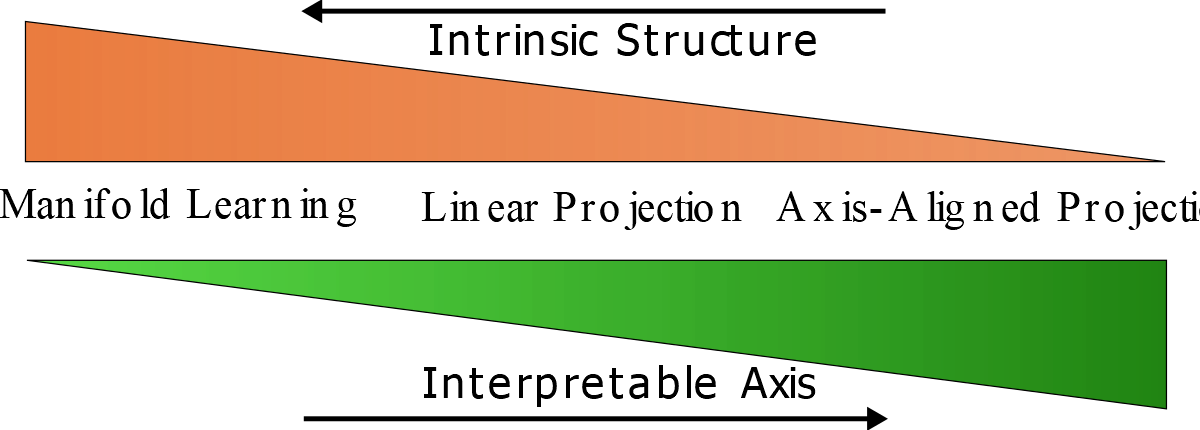
\includegraphics[width=0.85\textwidth]{figs/chap3/interpretableAxis}
  \caption[Interpretability of Dimensionality Reduction Techniques]{Though more advanced nonlinear methods are able to capture a wider variety of intrinsic structures of the data, they do so at the cost of interpretability. Reproduced from Liu et al.~\cite{LiuMaljovecWang2015}}
  \label{fig:axisInterpretability}
\end{figure}

\subsection{Visualizing Sensitivity}
\label{sec:SA_visualization}
Within the sensitivity literature visual representations conveying sensitivity information include a variant of the bar chart known as a tornado plot, parallel coordinate plots and their circular variant, the radar chart, scatterplot matrices,  and generalized reachable sets (GRS)~\cite{SaltelliChanScott2000,BushenkovChernykhKamenev1995}.

More recently, the visualization community has explored the use of glyphs to provide statistical and sensitivity information in order to present trends in the data.
%
By utilizing local linear regression to compute partial derivatives around sampled data points and representing the information in terms of glyph shape, sensitivity information can be visually encoded into scatterplots~\cite{CorreaChanMa2009,ChanCorreaMa2010,GuoWardRundensteiner2011,ChanCorreaMa2013}.

Correa et al.~\cite{CorreaChanMa2009} aimed at incorporating uncertainty information into PCA projections and k-means clustering and accomplished this goal by augmenting scatterplots with tornado plots.
%
Together these glyphs encode uncertainty and partial derivative information.
%
The idea of mapping sensitivity information to a line segment through each data point has been extended in their later work~\cite{ChanCorreaMa2010} with the introduction of the flow-based scatterplot (FBS) that highlights functional relationships between inputs and outputs.
%
The works by Guo et al.~\cite{GuoWardRundensteiner2011} and Chan et al.~\cite{ChanCorreaMa2013} attempt to provide more than a single partial derivative information into their scatterplots by experimenting with different glyph shapes such as star plots, among others.
%
Guo et al. also utilize a bar chart similar to the tornado plot used by Correa et al., whereas Chan et al. provide two other interpretations.
%
The first is a generalization of the FBS called the generalized sensitivity scatterplot (GSS).
%
By using orthogonal regression, GSSs can represent the partial derivative of any variable with respect to any other variable.
%
The other is a fan glyph that works similarly to the star glyph, allowing for viewing multiple partial derivatives, but rather than displaying magnitude as in the star glyph, the fan glyph highlights the direction of each partial derivative, since all line segments are normalized in length.

Several other visualization systems designed for SA also exist in the literature, some of which have been previously discussed in Section~\ref{sec:designSteering} and are repeated here for clarity.
%
Most of these systems enable visual exploration of local sensitivity information.

HDViz~\cite{GerberBremerPascucci2010} characterizes the behavior of system outputs with respect to input parameters geometrically.
%
HyperMoVal~\cite{PiringerBergerKrasser2010} highlights discrepancies occuring between the data and the model, and computes sensitivity information on the model.
%
The software proposed in Chapter~\ref{ch:visualization} provides similar capabilities by reporting on the fitness of each local regression model fit to a partition of the data.
%
Berger et al.~\cite{BergerPiringerFilzmoser2011} provide a focus+context display that provides local sensitivity information on and near a user-selected focal point.
%
Tuner~\cite{Torsney-WeirSaadMoller2011} allows users to explore sensitivity information through interaction and visual inspection, that is, by noticing which plots change the most when the user adjusts a parameter.
%
Demir et al.~\cite{DemirWestermann2013} utilize the HyperSlice~\cite{VanWijkVanLiere1993} technique to enhance the understanding of the sensitivity information provided by a Gaussian Process fit.
%
Vismon~\cite{BooshehrianMullrPeterman2012} provides SA to the visualization of the uncertainty of a simulation for fisheries scientists.

Canonical correlation analysis (CCA) was used in constructing the heliograph~\cite{DeganiShaftoOlson2006} and a system called Slycat~\cite{CrossnoSheadSielicki2015} to determine correlations between multiple inputs and multiple outputs in a global setting for ensemble data.

The proposed method given in Chapter~\ref{ch:visualization} is, in spirit, similar to systems provided in May et al.~\cite{MayBannachDavey2011} and Muhlbacher et al.~\cite{MuhlbacherPiringer2013}, by providing the capability to interactively refine the partitioning during the SA to give a multi-scale view of the sensitivity information.
%
However in both previous works, data is partitioned along one or two dimensions (i.e. input parameters) while the method presented in this dissertation spans all dimensions.

\section{Data Modeling}
\label{sec:regression}
\subsection{Parametric Regression}
\subsubsection{Linear Regression}
The most straightforward types of data modeling occur when the data can be well approximated in closed form by a linear or polynomial model.
%
For example, consider a problem with several independent variables, $x_i, i=1,...,d$, and one dependent variable, $y$.
%
We seek to capture the relationship between each $x_i$ and $y$ through linear relationships: $y = \beta_0 + \beta_1 x_1 + \beta_2 x_2 + ... + \beta_d x_d + \epsilon$, where $\epsilon$ represents random error.
%
This equation is given in intercept form where $\beta_0$ represents the y-intercept.
%
When the data is appropriately centered to have a mean of zero ($\mu_x,\mu_y = 0$), $\beta_0$ can be omitted.
%
For the remainder of this section, we will adopt the more flexible matrix notation where in intercept form, $\mathbf{X} = \begin{bmatrix}\mathbf{1} & \mathbf{x}_1 & \ldots & \mathbf{x}_d \end{bmatrix}$ such that the first column is a series of ones which will be multiplied by the y-intercept term, $\beta_0$, and the remaining columns are the input dimensions.
%
In the centered case, this notation is consistent, as we can drop the initial column in $\mathbf{X}$ such that $\mathbf{X} = \begin{bmatrix}\mathbf{x}_1 & \ldots & \mathbf{x}_d\end{bmatrix}$ and remove $\beta_0$ from the linear coefficient vector, $\boldsymbol\beta$.

Given a set of observations $(\mathbf{X},\mathbf{y})$, the problem in matrix form is given below:
%
\begin{equation}
\mathbf{y} = \mathbf{X}\boldsymbol\beta + \boldsymbol\epsilon
\end{equation}
%
In this equation, we seek to find a $\boldsymbol\beta$ that minimizes the error captured in $\boldsymbol\epsilon$.
%
Consider the proposed solution, $\tilde{y} = \mathbf{X}\mathbf{b}$.
%
We define the difference between our model evaluated at an input row $\mathbf{x}_j$ and the corresponding true response $y_j$ as the residual: $r_j = y_j - \mathbf{x}_j\mathbf{b}$.
%
This leads us to the least squares method which minimizes the sum of squared residuals over the entire observed data:
\begin{equation}
\arg\min_{\mathbf{b}} \sum_{j=0}^n(y_j - \mathbf{x}_j\mathbf{b})^2
\end{equation}

In order to minimize the sum of squared residuals, we can differentiate the sum of squared residuals equation with respect to each variable in $\mathbf{b}$ and set each derivative equal to zero.
%
Rearranging the terms leads to a series of \emph{normal equations}:
\begin{equation}
(\mathbf{X}^T\mathbf{y}= \mathbf{X}^T\mathbf{X}\mathbf{b})
\end{equation}

Thus, the solution to the least squares problem is:
\begin{equation}
\mathbf{b} = (\mathbf{X}^T \mathbf{X})^{-1} \mathbf{X}^T \mathbf{y}
\label{eq:ols}
\end{equation}

The case with a single input variable is called simple linear regression and the case where $d\geq 2$ is called multiple linear regression.
%
This method can also be extended to polynomials by treating each degree of a variable as separate columns in $\mathbf{X}$, and solving for additional coefficients for each term.
%
Similarly, the method can also be extended to mixtures of different variables of varying orders.
%
It is important to note, that this is the simplest version of linear and polynomial regression and more advanced methods can be performed.

The ordinary least squares method described above can fail if the problem exhibits collinearity.
%
Collinearity, or multicollinearity, occurs when two or more input variables are highly or perfectly correlated.
%
If perfectly correlated, the matrix in Equation~\ref{eq:ols} is less than full rank and cannot be inverted.
%
Similarly, if the variables are highly correlated, then the problem will be ill-conditioned.
%
In addition, overfitting can result if too many terms are included in the least squares problem.
%
To this end, processes such as regularization and variable selection can be employed to prevent these issues to some extent.
%
We review the more common techniques in the next section.

\subsection{Regularization and Feature Selection}
\label{sec:regularization}
Regularization is a generic concept that can be applied to any problem where the goal is to minimize a loss function.
%
Though regularization is not restricted to the linear regression problem, it expedites exposition to describe it in this context.
%
Regularization, in the regression setting posed, augments a minimization problem with a penalty function, $R$, that favors less complex models and a penalty term $\alpha$ that controls its influence on the solution.
%
In the context of our linear regression problem, we would have a new minimization problem resembling the one given below:

\begin{equation}
\arg\min_{\mathbf{b}} \sum_{j=0}^n(y_j - \mathbf{x}_j\mathbf{b})^2 + \alpha R(\mathbf{b})
\label{eq:genericRegularization}
\end{equation}

Common penalization functions include the $L_1$ and $L_2$ norms of $\mathbf{b}$ which result in the least absolute shrinkage and selection operator (LASSO)~\cite{Tibshirani1996} and ridge regression~\cite{Hoerl1959,Hoerl1962}, respectively.
%
The ridge regression methodology tends to include all of the original terms whereas the LASSO method tends to favor models with fewer parameters, i.e. one or more parameters of $\mathbf{b}$ are set to zero.
%
Zou and Hastie~\cite{ZouHastie2005} point out several disadvantages of the LASSO method, as well.
%
For example, the LASSO method tends to be over aggressive in its parameter selection in cases where the dimensionality is larger than the sample size or if two or more variables exhibit collinearity.
%
For this reason, they propose the elastic net method which combines the $L_1$ and $L_2$ norms to create a regularizer that counteracts the weaknesses of both ridge and LASSO regression.

Depending on the specific penalty function, regularization can also effectively remove parameters by forcing their coefficients in $\mathbf{b}$ to zero.
%
This is a form of feature or variable selection.
%
Variable selection is the process of eliminating redundant or irrelevant variables in order to construct a model that uses only a subset of the original input variables and this is only one way in which it can be performed.
%
Other methods for explicitly performing variable selection include stepwise regression~\cite{DraperSmith2014}, least-angle regression (LARS)~\cite{EfronHastieJohnstone2004}, and matching pursuit~\cite{MallatZhang1993,DavisMallatZhang1994,PatiRezaiifarKrishnaprasad1993}.
%
We briefly review them here.

Stepwise regression builds a regression model by iteratively adding or removing variables based on statistical testing that dictates how sensitive the model is to each variable.
%
In the additive model, the process begins with a single variable and adds additional variables until the gain in accuracy becomes negligible.
%
This process is known as forward selection.
%
Alternatively, one may begin with a model built on the full set of variables and iteratively remove variables until the model's accuracy degrades beyond an acceptable level.
%
This process is known as backward elimination.
%
A third class of methods called bidirectional elimination combines the processes of forward selection and backward elimination.

The LARS method is similar to the forward selection method above in that all coefficients of our model begin at zero and we add to the coefficients depending on their influence (correlation) on the response value.
%
Iteratively, we evaluate the residuals of the current model and increase the coefficient until another parameter becomes more correlated.
%
At this point, the direction of coefficient increase becomes equiangular between the two most correlated features.
%
This process continues adding coefficients to features as they become as correlated as the existing features in the model,
and we maintain a direction of travel that is equiangluar amongst the existing features.

Matching pursuit~\cite{MallatZhang1993} and its orthogonalized variant~\cite{DavisMallatZhang1994,PatiRezaiifarKrishnaprasad1993} are forward selection methods that either approximate an optimal minimum number of non-zero coefficients given an error tolerance, or minimize the error given a maximum number of non-zero coefficients.
%
The matching pursuit algorithm is a greedy iterative algorithm that was originally developed for compressed sensing.
%
At each step, the algorithm selects to include the coefficient associated to the variable that is most highly correlated to the residual of the current fit.
%
In the orthogonal version, all of the coefficients used so far are updated by computing the residual using an orthogonal projection on the subset of dimensions used.

\subsection{Partition-Based Models}
Thus far, we have discussed fitting a global model to a point cloud sampling of our domain of interest.
%
Such regression models are easily interpretable, although their application is somewhat limited.
%
Linear regression models are unable to capture non-monotonic behaviors, and unless the underlying degree of the function is known a priori, polynomial regression can overfit the data.
%
Of course, these effects can be mitigated if the data is partitioned appropriately.

Partition-based regression techniques typically employ a systematic domain partitioning based on various criteria, coupled with regression models fitted to each partition, to identify and understand local structures of the model.
%
They can be classified based on their partitioning criteria: those seeking to minimize numerical errors~\cite{Friedman1991,AlexanderGrimshaw1996,BreimanFriedmanOlshen1984a,ChaudhuriHuangLoh1994,ChipmanMcCulloch2010}, and those based on geometric analysis~\cite{GerberPotter2012,GerberRubelBremer2011,LiLueChen2000}.
%
In particular, regression trees are constructed by recursively partitioning the domain into multiple partitions at \emph{optimal} locations in the domain (where the optimal criteria can vary), and each partition is fitted with constant~\cite{BreimanFriedmanOlshen1984a}, linear~\cite{AlexanderGrimshaw1996,LiLueChen2000}, low-order spline~\cite{Friedman1991} or polynomial~\cite{ChaudhuriHuangLoh1994} models.

A popular class of regression tree is Friedman's multivariate adaptive regression splines (MARS)~\cite{Friedman1991} which is utilized in Section~\ref{paper:ijuq2013} (see also Hastie et al.~\cite{HastieTibshiraniFriedman2008} for a gentle introduction).
%
MARS is a non-parametric regression method that uses a collection of simple basis functions to build a complex and flexible response function.
%
At the core of MARS are piecewise linear basis functions, given by $\max(0, x - k)$ and $\max(0, k - x)$, where $k$ is the knot (the break point).
%
These simple functions are used to build a collection of basis functions, $\{\max(0, x_j-k), \max(0,k-x_j)\}$, where $k \in \{x_{1j}, \dots, x_{nj})$ for $j = 1, \dots, d$.
%
If all of the input values are different in the training data this will yield $2dn$ basis functions. The MARS predictor is then given by $\hat{y}(\mathbf{x}) = \beta_0 + \sum_{m=1}^M \beta_m h_m(\mathbf{x})$, where the $\beta_m$'s are coefficients and the $h_m$'s are basis functions, which are either given by a single function from the collection of simple basis functions or a product of
two or more of such functions.

For a given set of basis functions, $h_1, \dots, h_m$, the $\beta$ coefficients are estimated using least squares.
%
The main novelty of the MARS is how the basis functions are selected using a forward selection process, followed by a backward elimination process.
%
The forward pass starts with a model that only includes the constant term $\beta_0$ and then adds simple basis functions in pairs in a greedy fashion.
%
This yields a model that over fits the training data (i.e.\ has too many terms).
%
The backward elimination process drops terms using the generalized cross-validation (GCV) criterion, which compromises between the fidelity of the model and its complexity (size).

As with most non-parametric regression methods, there is no direct method to assess their prediction error.
%
However, the prediction error can be estimated by bootstrap methods~\cite{DavisonHinkley1997}.
%
In short, an ensemble of MARS models is created by repeatedly resampling, with replacement, the original training data $\{ (\mathbf{x}_i, y_i) \}$ and a MARS model is fit to each batch of resampled data.
%
An estimate of the prediction error is then given by the standard deviation of the predictions provided by the bootstrap ensemble.
%
This method is employed for adaptive sampling using a MARS model in Section~\ref{paper:ijuq2013} in order to define several of the scoring functions when using a MARS model.

In terms of more geometrically motivated splitting criteria, the principal Hessian direction regression tree (PHDRT)~\cite{LiLueChen2000} splits the domain near areas of high curvature by projecting the data along its estimated principal Hessian direction and locating the area of highest curvature.
%
In Chapter~\ref{ch:visualization}, we employ the established Morse-Smale regression (MSR)~\cite{GerberRubelBremer2011}, which, being geometrically motivated, is similar to the PHDRT approach, however it is not restricted to splitting along a hyperplane and is also more robust to multiple undulations in the data.
%
In the PHDRT approach, a mean principal Hessian direction is computed implying that positive and negative curvatures can have a canceling effect that prevents such a direction from being discovered.

MSR utilizes a domain partitioning induced by the Morse-Smale complex (MSC) of the regression surface.
%
The MSC partitions the domain into monotonic regions, and MSR takes advantage of the monotonicity implied by this partitioning and builds linear models to fit each partition to capture local interactions between input and output parameters.
%
The MSC is at the core of the HDViz visualization system~\cite{GerberBremerPascucci2010}.
%
HDViz has been extended in order to apply it to the analysis of data in nuclear engineering~\cite{MaljovecLiuWang2015,MaljovecWangMandelli2013a,MaljovecWangPascucci2013}.
%
However, the insights made by nuclear scientists were limited by the complexity and the lack of intuition provided in the original visualization.
%
In the new research of Chapter~\ref{ch:visualization}, we follow an iterative process of designing and refining a new visualization system, using HDViz as a basis, that specifically targets nuclear scientists as end users and sensitivity analysis as the end task.
%
% Section~\ref{paper:vis2016} discusses in more detail the drawbacks of both PHDRT and MSR and proposes the construction of a hybrid method that uses the benefits of both in order to better characterize complicated datasets.

\subsection{Neural Networks}

The combination of accessibility to cloud computing architectures, large-scale data collection/storage, and advancements in GPU processing have made neural networks and deep learning both feasible and widely available.
%
As a result, they have gained immensely in popularity due to the universal approximation theorem~\cite{Cybenko1989,Funahashi1989,Hecht-Nielsen1987,HornikStinchcombeWhite1989}.
%
Without first introducing the mathematical formulation of a simple neural network, we can summarize the most generic form of the universal approximation theorem as stating that a neural network with a single hidden layer containing a finite set of neurons defined over a compact set in $\mathbb{R}^n$ is capable of approximating a continuous function to within a given $\epsilon$ error under mild assumptions on the formulation of the artificial neurons.
%
Several authors have proven this empowering theorem under various circumstances~\cite{Hornik1991,Hornik1993,Huang2003,HuangBabri1998,IrieMiyake1988,Kurkova1992,LeshnoLinPinkus1993,ParkSandberg1991} (see the survey by Scarselli and Tsoi for a more complete list~\cite{ScarselliTsoi1998}), however caveats still remain.

The universal approximation theorem does not state the exact size/complexity required to attain a specific level of approximation nor that an algorithm exists that will converge to this theoretical existent model.
%
For these reasons and the lack of interpretability of such complicated models, some researchers are still slow to adopt these methods.
%
Deep learning algorithms are still largely considered a black-box solution to a problem since it difficult to trace the result of a prediction to a specific collection of neurons/coefficients especially those with several layers of abstraction.
%
Nonetheless, empirically they have proven successful as predictors on many datasets in varied domains such as image analysis~\cite{Daugman1988,FarabetCouprieNajman2012,HadsellSermanetPierre2009,KrizhevskySutskeverHinton2017,MillertariNavabAhmadi2016,YasminSharifMohsin2013}, text, speech, and natural language processing~\cite{BengioDucharmeVincent2003,GravesMohamedHinton2013,GravesWayneDanihelka2014,HochreiterSchmidhuber1997,MaPrincipe2018,SutskeverVinyalsLe2014,WestonBordesChopra2015}, graph-based problems~\cite{WuPanChen2019,ZhangCuiZhu2018,ZhouCuiZhang2018}, and even outperforming humans in complex games~\cite{MnihKavukcuogluSilver2013,SilverHuangMaddison2016}.

To introduce the topic, I will explain a simple feed-forward neural network with a single hidden layer that we can later generalize to more arbitrarily complex models.
%
For further details, I defer to Ripley~\cite{Ripley1996} and Hastie et al.~\cite{HastieTibshiraniFriedman2008} for more in-depth analysis.

An artificial neural network is modeled after neural networks seen in biology such as our own nervous system.
%
The idea is to view the data as being layered, where the model inputs and outputs comprise the two outermost layers which are connected by a pathway of one or more ``hidden'' layers that models how input signals are transmitted through a pathway of neurons in order to solve a problem or make a decision.
%
In its simplest form, a single hidden layer is comprised of artificial neurons which each perform a different operation on the incoming data and pass that information to the output layer.
%
The artificial neurons are trained and their connections from the input layer and to the output layer are inhibited or enforced depending on the training data.
%
Below, I will describe more mathematically how this can occur in order to produce a usable result.

The single layer neural network is a non-linear statistical model, where the response of interest is modeled as a linear combination of $M$ derived features (the hidden units of the neural network):

\begin{equation}
\hat{y}(\mathbf{x}) = \beta_0 + \boldsymbol{\beta}^T \mathbf{z}
\end{equation}

where $\mathbf{z} = (z_1, \dots, z_M)^T$ and $z_m = \sigma(\alpha_{0m} + \boldsymbol{\alpha}_m^T \mathbf{x})$.
%
$\sigma(v)$ is known as the activation function and using the neural pathway example is responsible for activating/propagating a signal or quelling it.
%
It works by mapping a real-valued scalar value onto a desired range which may or may not be bounded depending on the application.
%
Example activations include the sigmoid function, $\sigma(v) = 1/(1+e^{-v})$, the hyperbolic tangent function, $\sigma(v) = \frac{e^v-e^{-v}}{e^v+e^{-v}}$, the rectified linear unit, $\sigma(v) = \max(0, v)$, and the leaky rectified linear unit, $\sigma(v) = \max(\epsilon v, v)$, where $\epsilon \ll 1$.
%
The unknown parameters of the neural network, which we denote by $\boldsymbol{\theta}$ are often referred to as weights, and consist of the $M(d+1)$ $\alpha$'s of the hidden layer and the $M+1$ $\beta$'s for the response model.
%
The weights are estimated by minimizing the sum-of-squares, $R(\boldsymbol{\theta}) = \sum_{i=1}^n (y_i - \hat{y}(\mathbf{x}_i))^2$.
%
However, for a large neural network, the resulting neural network over-fits the data (i.e., the neural network fits the training data well, but performs poorly on independent validation data).
%
A common solution is to add a regularization term that shrinks the weights to zero, such as $J(\boldsymbol{\theta}) = \sum_{m=0}^M \beta_{m}^2 + \sum_{m=0,j=1}^{M,d} \alpha_{mj}^2$, and then minimize $R(\boldsymbol{\theta}) + \lambda J(\boldsymbol{\theta})$.
%
The minimization can be carried out in an efficient manner using gradient-based methods, as the gradient of the neural network can be computed easily using the chain rule for differentiation.
%
As in the case of MARS, the prediction error of the neural network can be estimated using bootstrap methods.

\subsection{Support Vector Machines}
\label{sec:svm}

Support Vector Machines (SVMs) were first introduced as a means of binary classification via a linear separator~\cite{VapnikLerner1963}.
%
In the classical case, a hyperplane is used to divide two classes of points where a subset of the original data is used to determine this hyperplane.
%
The specific subset of data used are known as the \emph{support vectors} and can intuitively be thought of as the points closest to the boundary separating the two classes.
%
Using the support vectors, we can construct the equation of the separating hyperplane, $S_0: 0 = \mathbf{w} \cdot \mathbf{x} - b$ by constructing an optimality criteria that the hyperplane has a maximal distance to the support vectors and the fewest number of misclassified points (in the case where the data is not linearly separable).
%
Figure~\ref{fig:svmExample} shows an annotated example of the support vector machine applied to a dataset that is linearly separable.

\begin{figure}[!ht]
  \centering
  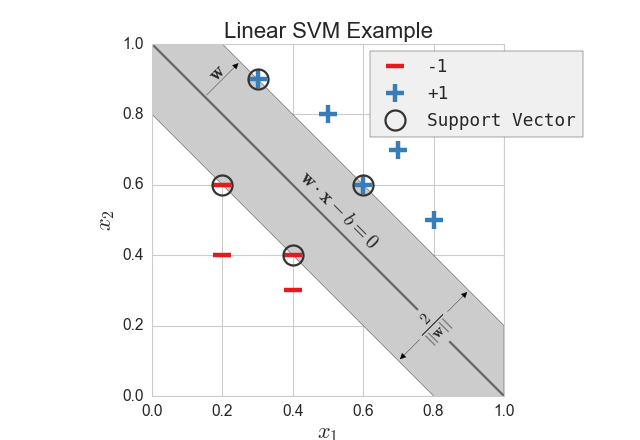
\includegraphics[width=0.85\textwidth]{figs/chap3/svmExample}
  \caption[Linear Support Vector Machine Example]{A two-dimensional example dataset showing the linear separator, margin, and support vectors of a trivial classification problem.}
  \label{fig:svmExample}
\end{figure}

We can see from Figure~\ref{fig:svmExample} that the support vectors of each class define hyperplanes that are parallel to $S_0$, namely $S_{-}$ and $S_{+}$ which are set to be defined by the equations $-1 = \mathbf{w} \cdot \mathbf{x} - b$ and $1 = \mathbf{w} \cdot \mathbf{x} - b$, respectively.
%
The shaded region bounded by the separating hyperplanes, $S_{-}$ and $S_{+}$, is known as the \emph{margin} and represents the area we seek to maximize.
%
The width of the margin is inversely proportional to the norm of the separating hyperplane coefficients, $\mathbf{w}$.
%
Therefore, by minimizing $||\mathbf{w}||$ according to the constraint that our data lies on the correct side of the margin, we obtain the optimal separating hyperplane.

If we define our class labels to be $y_i: y_i \in \{-1,1\}$, then we can rewrite the constraints in a single equation: $y_i(\mathbf{w} \cdot \mathbf{x_i} - b ) \geq 1$ for $i=1,...,n$ where $n$ is the number of support vectors.
%
In the case where the data is not linearly separable in the original space, we can either relax our constraint to include a soft margin that allows points to be misclassified~\cite{CortesVapnik1995} and/or the data can be transformed into a feature space where it is linearly separable~\cite{BoserGuyonVapnik1992}.

The formulation of the SVM can also be augmented to work in a regression setting, however this is beyond the scope of this work, and so the interested reader is referred to the work of Drucker et al.~\cite{DruckerBurgesKaufman1997} for more details regarding that formulation.

\subsubsection{Soft Margin SVM}

To instantiate a soft margin, we replace the constraint function with a loss function so that our optimization problem penalizes equations that misclassify points.
%
The \emph{hinge loss} function is often used for such purposes, and it is defined in Equation~\ref{eq:hingeLoss}.
%
\begin{equation}
l(\mathbf{x_i},y_i) = \max(0,1-y_i(\mathbf{w} \cdot \mathbf{x_i} - b))
\label{eq:hingeLoss}
\end{equation}
%
Note that for correctly classified data, the hinge loss function will return zero and the value increases the farther a misclassified point is from $S_-$ (for $y_i=-1$) or $S_+$ (for $y_i=1$).
%
We then combine this hinge loss over all of the support vectors with the original minimization criteria on $||\mathbf{w}||$ to give the minimization problem in Equation~\ref{eq:svmSoftMargin}.
\begin{equation}
\argmin_{\mathbf{w},b}\frac{1}{n}\sum_{i=1}^n \left(l(\mathbf{x_i},y_i)\right) + \lambda ||\mathbf{w}||^2
\label{eq:svmSoftMargin}
\end{equation}

The $\lambda$ in the above optimization represents a postive real number and allows a user to appropriately weight how important the size of the margin should be in comparison to the correctness of classification.
%
As $\lambda$ decreases in magnitude, the behavior of the SVM will tend toward the hard-margin case described above.

\subsubsection{Kernel SVM}

Consider the example shown in Figure~\ref{fig:kernelSvmExample}.
%
The image on the left represents the data in the original data space, and it is clear that there does not exist a line that can separate the two classes.
%
However, we can note that by applying a transformation operator, $K$ on the original data, we can transform it into a space where the data is linearly separable as shown in the right image.
%
In this case, we have kept the dimensionality the same ($d=2$), but we have transformed our cartesian coordinates ($x_1$ and $x_2$) into polar coordinates ($r$ and $\theta$).
%
This is the main concept behind kernel-based SVMs where often the data is projected into a higher dimensional feature space.

\begin{figure}[!ht]
  \centering
  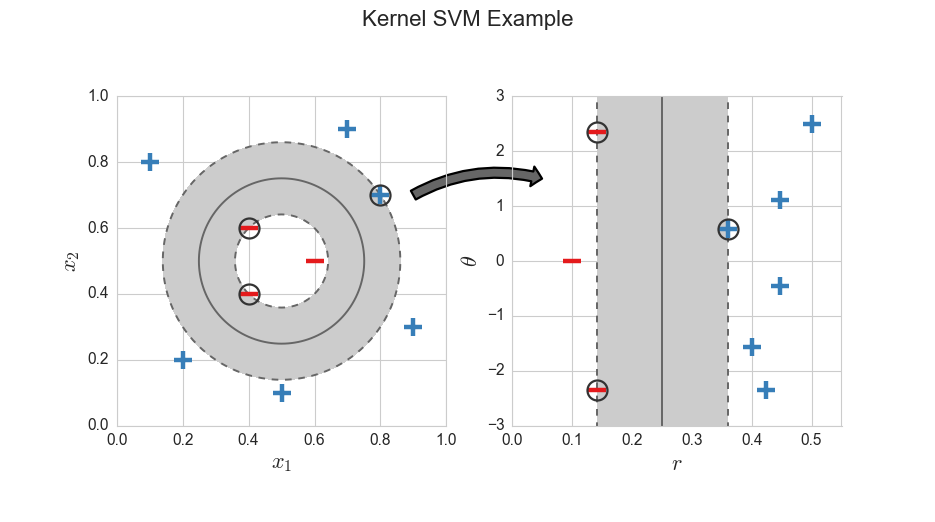
\includegraphics[width=0.85\textwidth]{figs/chap3/kernelSvmExample}
  \caption[Kernel Support Vector Machine Example]{A two-dimensional example dataset is transformed into a different space where it can be linearly separated and the support vector algorithm acts on the transformed space.}
  \label{fig:kernelSvmExample}
\end{figure}

When applying a kernel on the data, the same optimization process can be applied in the higher dimensional feature space in order to determine the maximum-margin linear separator in the feature space~\cite{BoserGuyonVapnik1992}.
%
Common kernels include polynomial, radial basis, sigmoid, and hyperbolic tangent functions.
%
It should be noted that as opposed to transforming the data into a fixed dimension space these methods instead transform the data into a feature space whose dimensionality is dependent on the number of training samples.

The resulting optimization problem of all of the described SVM methods is $\mathcal{O}(n^2)$ with respect to the training size and the computation time is not affected by the dimensionality of the original space.
%
However, it is worth noting that as dimensionality increases, the out-of-sample error can become a problem which requires more training data to counterbalance.

\subsubsection{SVM Approximations and Optimizations}

Various improvements have been made to optimize the computation costs of the support vector machines, many of these are summarized by Shawe-Taylor and Sun~\cite{Shawe-TaylorSun2011}.
%
The techniques can be broadly classified into a few categories.
%
Ther first of these formulates the SVM as a quadratic programming problem and uses the well-established interior point algorithm~\cite{BoydVandenberghe2004,FineScheinberg2002,FerrisMunson2002,ScholkopfSmola2001}.
%
Such methods are efficient and provide reliable and precise solutions for smaller sized problems.
%
The second category of methods decompose the problem into smaller subproblems either by chunking~\cite{BordesErtekinWeston2005,ChangLin2011,Joachims1999,OsunaFreundGirosi1997,Platt1998,Vapnik1982,ZanniSerafiniZanghirati2006} or by employing an active set strategy~\cite{CauwenberghsPoggio2000,HastieRossetTibshirani2004,Scheinberg2006,ShiltonPalaniswamiRalph2005}.
%
% Chunking the SVM problem into smaller subproblems where solutions of the subproblems are retained speeds up the computation of the larger problem until all of the training data has been used~\cite{OsunaFreundGirosi1997,Vapnik1982}.
% %
% Platt used this methodology in his sequential minimal optimization (SMO) solution that exploits the analytic solution of the case with two training points thus avoiding the need of a numerical solver~\cite{Platt1998}.
%
% Bordes et al.~\cite{BordesErtekinWeston2005} provide an online implementation called LASVM that makes a sequential pass through the current training data in
% order to reorganize the SMO solution and provide even further improvement.
%
A third category instead looks at decomposing the problem by focusing on one
coordinate or parameter at a time~\cite{BordesBottouGallinari2007,FriessCristianiniCampbell1998,HsiehChangLin2008,MangasarianMusicant1999}.

Whereas the aforementioned methods formulate a dual problem there are some methods which instead focus on solutions to the primal problem which can be more easily optimized and in some cases handling approximate solutions~\cite{BottouBousquet2008,Shalev-ShwartzSingerSrebro2011}.
%
These optimizations include using Newton's method~\cite{Chapelle2007,KeerthiDeCoste2005,LeeMangasarian2001,Mangasarian2002}, stochastic sub-gradients with projection~\cite{KivinenSmolaWilliamson2004,Shalev-ShwartzSingerSrebro2011,Zhang2004}, and cutting plane methods~\cite{FrancSonnenburg2008,Joachims2006,TeoSmolaVishwanathan2007}.
%
The latter two methods are capable of handling non-differentiable objective functions.

\subsection{Bayesian Methods}

Bayesian techniques can also be used to model the problems described herein, but focus on \emph{inference}.
%
In these methods, a prior distribution is employed before sampling to express the belief about the shape of the data.
%
There is a rich body of work that discusses these techniques, but for an overview discussion, see MacKay~\cite{MacKay1992b}.
%
Of particular interest is the Gaussian process (GP) model~\cite{RasmussenWilliams2006}.

GP regression, or Kriging~\cite{Stein1999}, is a response surface method that assumes a field of random variables where any finite collection of variables can be considered to follow a joint Gaussian distribution.
%
Thus, any finite collection of data (read training data) can be modeled as a multivariate normal distribution over functions.
%
As such a GP can be characterized on a dataset through the use of a mean and covariance function.
%
Kriging provides a \emph{best unbiased linear prediction} for unobserved locations by averaging a neighborhood of points around the query location weighted by a mean and covariance function.

The response variable, $y=f(x)$ at any arbitrary location $z$ has a normal probability distribution given in Equation~\ref{eq:gp} where $X$ is a given $n \times d$ design matrix of inputs, $m(X) = \mu_y$ is the expected value of an associated given output vector of size $n$.

\begin{equation}
p(f(z)|X,y) = \mathcal{N}(m(X),k(X,z))
\label{eq:gp}
\end{equation}

Often the mean function is assumed to be zero which can simplify the computation and can be done without loss of generality~\cite{Seeger2004}.

\begin{equation}
p(f(z)|X,y) = \mathcal{N}(0,k(X,z))
\label{eq:gpSimple}
\end{equation}

Of general importance are the mean and variance prediction at an arbitrary location and the equations for computing these are shown below.

\begin{eqnarray}
\mu(z|X,y) & = & k(X,z)k(X,X)^{-1}y\\
\sigma(z|X,y) & = & k(z,z) - k(X,z)k(X,X)^{-1}k(X,z)^T
\end{eqnarray}

Note, $k(X,X)$ denotes a matrix of all possible covariances of the input samples, $k(X,z)$ represents a vector of the covariances of each input sample with the query location $z$.

From Equation~\ref{eq:gpSimple}, the user needs only to select a covariance function to use and then set the value of its hyperparameters, in order to query a GP at an arbitrary location.
%
As the covariance function works to weight the contribution of a neighboring point's influence on the prediction of a query location, it makes sense to have a function that is maximal at the query location and tends to zero as the distance from the query location grows.
%
Thus, it is common to see kernel functions used such as the squared exponential (most common), linear, piecewise polynomial, Mat\'{e}rn, and the Ornstein-Uhlenbeck functions, although any positive semidefinite function can be used in theory~\cite{RasmussenWilliams2006}.

From a supervised learning perspective, where the model should be ``fit'' to the training data, we fit hyperparameters to a prior covariance function defined for the data which allows us to make predictions on the data.
%
Various methods for fitting these hyperparameters exist such as cross validation and maximization of the marginal likelihood (see Chapter 5 of Rasmussen and Williams~\cite{RasmussenWilliams2006}).
%
The training process involves optimizing hyperparameters which are parameters to the selected covariance function.

\section{Topological Data Analysis}
A crucial step in gaining insights from large, complex, high-dimensional data involves feature abstraction, extraction, and evaluation in the spatiotemporal domain for effective exploration and visualization.
%
Topological data analysis (TDA, see~\cite{EdsbrunnerHarer2010,Zomorodian2005,BiasottisDeFlorianiFalcidieno2008,Carlsson2009,EdelsbrunnerHarer2008,Ghrist2009} for seminal works and surveys), has provided efficient and reliable feature-driven analysis and visualization capabilities.
%
Previous work in pure mathematical fashion has focused on the study of topological spaces under smooth and continuous settings without computational considerations of noisy and discrete datasets.
%
TDA typically operates under the discrete setting where combinatorial structures such as graphs or simplicial complexes are imposed on the point cloud data to approximate their underlying structure.
%
In Chapters~\ref{ch:adaptiveSampling}-~\ref{ch:graphs}, we apply TDA-based methods to different tasks in the design and analysis of computer experiments framework.
%
As such, we review the applications of TDA specifically for multidimensional data analysis and visualization.
%
A specific emphasis is placed on constructs from Morse theory as they operate specifically on scalar and vector function data.

Many TDA techniques construct topological structures~\cite{Reeb1946,Smale1961} from scalar functions on point clouds (e.g., Morse-Smale complexes, contour trees, and Reeb graphs) as ``summaries'' over data.
%
Among the commonly used TDA approaches, Reeb graphs/contour trees capture very different structural information of a real-valued function compared to extremum graphs and Morse and Morse-Smale complexes as the former is contour-based and the latter is gradient-based (Fig.~\ref{fig:topo-structure}).

\begin{figure}[!ht]
  \centering
  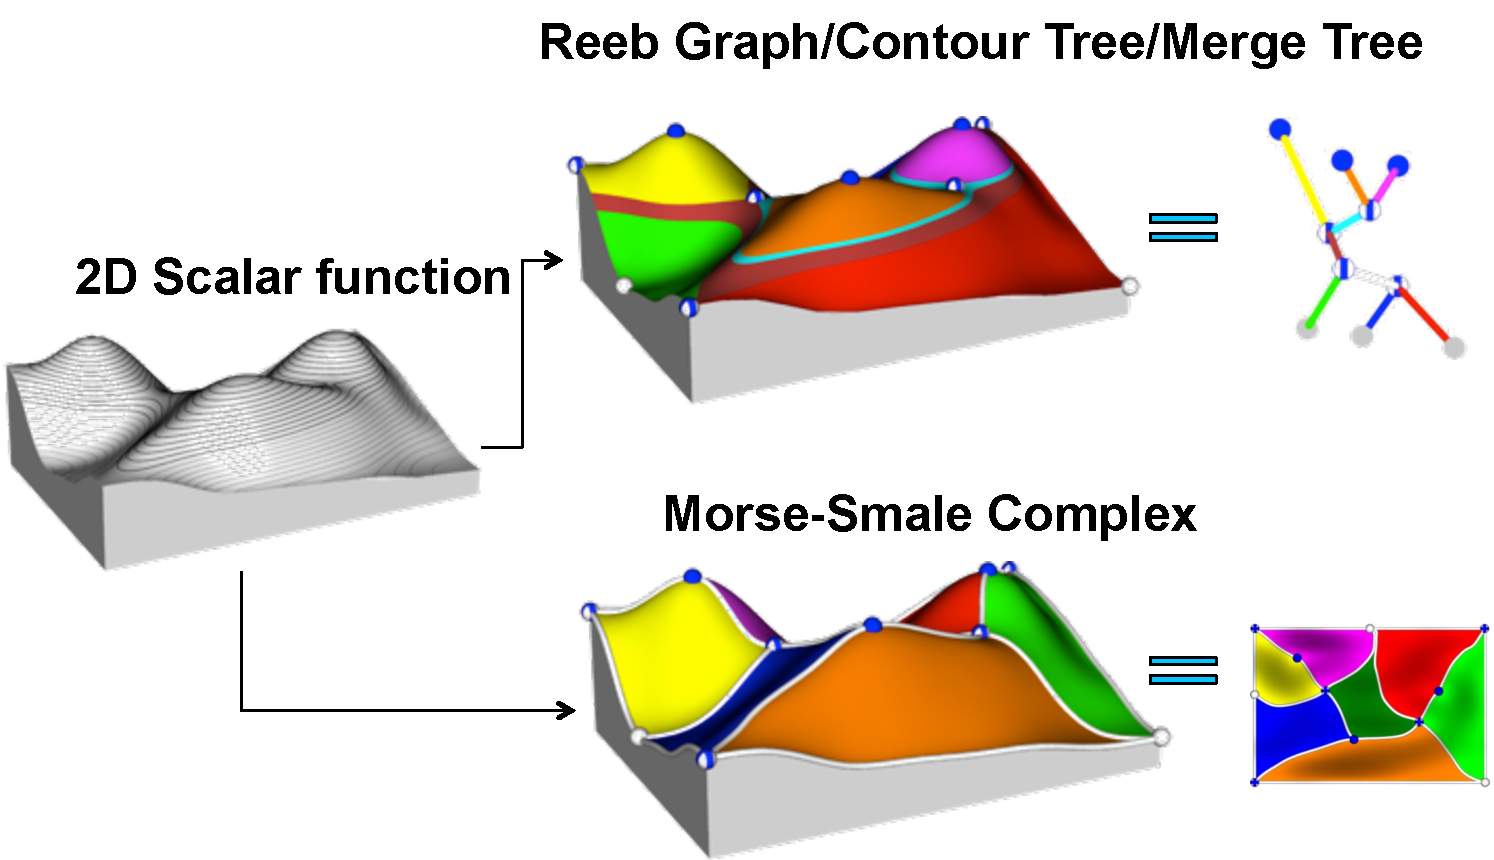
\includegraphics[width=0.85\textwidth]{figs/chap3/topostructure}
  \caption[Contour and Gradient-based Structures]{Contour- and gradient-based
  topological structure of a 2D scalar function.}
  \label{fig:topo-structure}
\end{figure}

They both provide meaningful abstractions of high-dimensional data, which reduces the amount of data needed to be processed or stored; and they utilize sophisticated hierarchical representations that capture features at multiple scales, which enables progressive simplifications of features differentiating small- and large-scale structures in the data.

\subsection{Gradient-Based Partitioning}
The Morse-Smale complex (MSC)~\cite{EdelsbrunnerHarerNatarajan2003,EdelsbrunnerHarerZomorodian2003} describes the topology of a function by clustering the points in the domain into regions of monotonic gradient flow, where each region is associated with a sink-source pair defined by local minima and maxima of the function.
%
The MSC can be represented using a graph where the vertices are critical points, and the edges are the boundaries of areas with similar gradient behavior.
%
The simplification of the MSC is obtained by removing pairs of vertices in the graph and updating connectivities among their neighboring vertices, thus merging nearby clusters by redirecting the gradient flow~\cite{ComicDeFloriani2011,GuntherReininghausSeidel2013,IuricichFugacciDeFloriani2015}.
%
MSCs have been shown to be effective in identifying, ordering, and selectively removing features of large-scale data in scientific visualizations (e.g.,~\cite{BremerEdelsbrunnerHamann2004,GyulassyBremerPascucci2008,GyulassyNatarajanPascucci2005}).

HDViz~\cite{GerberBremerPascucci2010}, mentioned previously, employs an approximation of the MSC (in high dimensions) to analyze scalar functions on point cloud data.
%
It creates a hierarchical segmentation of the data by clustering points based on their monotonic flow behavior, and designs new visual metaphors based on such a segmentation.
%
Correa and Lindstrom~\cite{CorreaLindstrom2011} suggest that by considering a different type of neighborhood structure, the accuracy in the extracted topology can be improved compared to those obtained within HDViz which relies on a $k$-nearest neighborhood which can tend to bias specific directions when the sampling density is variable across the domain.
%
Namely, they leverage a family of graphs known as empty region graphs which were introduced in Section~\ref{sec:graphs} and are discussed in greater detail in Section~\ref{sec:approximationMSC} and Chapter~\ref{ch:graphs}.
%

The topological spine~\cite{CorreaLindstromBremer2011} uses the Morse-Smale complex to build an extremum graph that can more faithfully represent complex structures such as cycles and fractals occurring in the topology.
%
Narayanan et al.~\cite{NarayananThomasNatarajan2015} design a metric for comparing such extremum graphs of related data that was used in time-varying data to identify significant events and periodicity in data.

\subsection{Levelset topology}

One use of Morse theory is to study the evolution of levelsets, that is the birth and death of connected components.
%
In order to conceptualize this idea, consider the manifold under study as a terrain and the Morse function value as the elevation of the terrain.
%
As we begin flooding the terrain, features will disappear, split, or develop holes.
%
Incidentally, each of these topology changing events can be modeled by studying the critical points of the manifold.
%
This concept was studied and formalized into such concepts as the Reeb graph and contour tree described below.

% \subsection{Reeb Graph}
The formal definition of the Reeb graph is given here:

\begin{defn}
\textbf{Reeb Graph} - The quotient space of the graph of $f$ in
$\mathbb{M} \times \mathbb{R}$ defined by the equivalence relation
$(\mathbf{x_i},f(\mathbf{x_i})) \sim (\mathbf{x_j},f(\mathbf{x_j}))$ iff
$f(\mathbf{x_i}) = f(\mathbf{x_j})$ and $\mathbf{x_i}$,$\mathbf{x_j}$ are part
of the same connected component of $f^{-1}(f(x_i))$, where $f : \mathbb{M} \rightarrow \mathbb{R}$ is a scalar function defined on a compact manifold, $\mathbb{M}$.
\end{defn}

Informally, the Reeb graph is the result of contracting each connected component of a levelset to a point and connecting corresponding points between levelsets via edges.
%
As stated above, it is only necessary to represent the levelsets of the critical points as nodes in the graph, and thus allow the edges of the graph to represent the infinite number of levelsets existing between critical points.

Georges Reeb, a French mathematician, first formalized the toplogical construct now known as the Reeb Graph in 1946~\cite{Reeb1946}.
%
The Reeb graph remained an abstract mathematical construct until 1991 when Shinagawa et. al.~\cite{ShinagawaKuniiKergosien1991} formalized and extended the necessary concepts from Morse theory to construct Reeb graph visualizations for reconstructing 3D surfaces from 2D cross sections.
%
Edelsbrunner et al.~\cite{EdelsbrunnerHarerMascarenhas2008} presented an improved algorithm for constructing a time-varying Reeb graph for the triangulated piecewise linear case of the Reeb graph and employed it for analysis of a function defined on a 3-sphere with no boundary.
%
Pascucci et al.~\cite{PascucciScorzelliBremer2007} later developed an online algorithm for efficiently constructing the Reeb graph on streaming data and prove its correctness on data of arbitrary dimensionality.
%
The survey of Biasotti et. al. gives a more thorough history of the Reeb graph, its theoretical considerations, and various applications~\cite{BiasottiGiorgiSpagnuolo2008}.

% \nb{Insert reeb graph example}

The Reeb graph of a real-valued function describes the connectivity of its level sets and has several related structures that are worth noting.
%
A contour tree is a special case of the Reeb graph that arises in simply connected domains.
%
A merge tree, also known as a barrier tree, is similar to Reeb graphs and contour trees except that it describes the connectivity of sublevel sets rather than level sets.
%
Efficient algorithms for computing the contour tree~\cite{CarrSnoeyinkAxen2003,ChiangLenzLu2005} and merge tree~\cite{OesterlingHeineWeber2015} in arbitrary dimensional spaces exist.

Mapper~\cite{SinghMemoliCarlsson2007} is a software tool that decomposes data into a simplicial complex resembling a generalized Reeb graph and visualizes the data using a graph structure with varying node sizes.
%
The software has been shown to extract salient features in a study of medical data by correctly classifying normal patients and patients with two different causes of diabetes~\cite{SarikondaPettusPhatak2014}.
%and various other applications~\cite{SchwartzFriedbergIvanov2012,KnightDavidsonHerman2014}.
%
It is shown, in a restrictive sense, that Mapper converges to the Reeb space (a higher-dimensional generalization of Reeb graph) in the limit~\cite{MunchWang2016}.
%
To this end, there have been some very recent efforts in understanding Reeb spaces and fiber surfaces via visualization, although those works have largely focused on bivariate functions on tetrahedral meshes~\cite{CarrGengTierny2015,KlacanskyTiernyCarr2016,TiernyCarr2016}.
%
Extensions of these works to general dimensionality are an open and interesting avenue of future research.

In terms of comparing the topologies of related data, the bottleneck distance between persistence diagrams is a well-established technique~\cite{Cohen-SteinerEdelsbrunnerHarer2007}, but Beketayev et al.~\cite{BeketayevYeliussizovMorozov2014} have recently devised a more robust metric for comparing merge trees that accounts for the nesting structure of the tree.

% \subsection{Contour Tree}

For the special case, where the Reeb graph is defined over a simply connected Euclidean space $\mathbb{E}^n$, we acheive the \textbf{contour tree}, that is a Reeb graph with no cycles and consisting of one connected component.
%
Carr et al.~\cite{CarrSnoeyinkAxen2003} introduced the first algorithm for computing the contour tree in any dimension.
%
Chiang et al.~\cite{ChiangLenzLu2005} sought to improve on Carr's method by avoiding the need to sort the entire dataset thus creating an output sensitive algorithm that only sorts subsets of the data.
%

Various visual metaphors have been designed for contour trees~\cite{PascucciCole-McLaughlinScorzelli2009,WeberBremerPascucci2012}.
%
In particular, variations of topological landscapes have been used extensively~\cite{BeketayevMorozovWeber2012,DemirBeketayevWeber2012,HarveyWang2010,OesterlingHeineJanicke2010,OesterlingHeineJanicke2011,WeberBremerPascucci2007}.
%
These visual metaphors have, or potentially have, capabilities for the visualization of high-dimensional datasets.
%
In particular, Weber et al.~\cite{WeberBremerPascucci2007} have presented such a metaphor for visually mapping the contour tree of high-dimensional functions to a 2D terrain where the relative size, volume, and nesting of the topological features are preserved.
%
Harvey and Wang~\cite{HarveyWang2010} have extended this work by computing all possible planar landscapes, and are able to preserve exactly the volumes of the high-dimensional features in the areas of the terrain.
%
In addition, the works of Oesterling et al.~\cite{OesterlingHeineJanicke2010,OesterlingHeineJanicke2011} have used this same metaphor to visualize a related structure, the join tree.
%
This collection of work uses a novel high-dimensional interpolation scheme in order to estimate the density from the raw data points and visually map the density as points on top of their generated terrains.

Oesterling et al.~\cite{OesterlingHeineGunther2013} continued this line of work by creating a linked view software system including user interactions into the analysis by allowing users to brush and link with parallel coordinate plots and PCA projections of the data.
%
In addition, they have presented a new method of sorting the features based on either persistence, cluster size, or cluster stability, thus adjusting the placement of features in the topological landscape.

% \begin{itemize}
% \item \cite{TiernyGyulassySimon2009}
% \item \cite{ChenObermaierHagen2012,ChenObermaierHagen2013}
% \item Go through TopoInVis, SOCG, SODA
% \end{itemize}

The Reeb graph and its relatives all store information regarding the number of components at any function value as well as how these components split and merge as the function value changes.
%
Such an abstraction offers a global summary of the topology of the level sets and enables the development of compact and effective methods for modeling and visualizing scientific data, especially in high dimensions (i.e.,~\cite{SinghMemoliCarlsson2007,NicolauLevineCarlsson2011}).

\subsection{Multifield Analysis}

The methods mentioned above deal primarily with scalar field data (except for those regarding Reeb spaces~\cite{MunchWang2016,CarrGengTierny2015,KlacanskyTiernyCarr2016,TiernyCarr2016}), but more recently techniques have been developed to also deal with multi-field data.
%
Jacobi sets~\cite{EdelsbrunnerHarer2002} have been used to locate the critical points of one scalar field restricted to the level sets of another scalar field, allowing for the simultaneous comparison of two variables of interest.
%
However, most applications of Jacobi sets have been to low-dimensional examples and are restricted to comparing only two outputs of interest.

A more recent and general technique is the development of the Joint Contour Net (JCN), a generalization of the Reeb graph introduced by Carr et al.~\cite{CarrDuke2014,DukeCarrKnoll2012} that allows for the analysis of multifield data.
%
Duke and Hosseini~\cite{DukeHosseini2015} have subsequently improved the performance with a parallel implementation of the JCN, and Geng et al.~\cite{GengDukeCarr2015} have improved the interactivity by enabling brushing and linking and demonstrated its effectiveness in finding periodic patterns in oceanic data.
%
Chattopadhyay et al.~\cite{ChattopadhyayCarrDuke2014,ChattopadhyayCarrDuke2016} have focused on bridging the gap between approximation and theory and produced an algorithm for performing simplification on the JCN among several other theoretical advancements.


The notion of Pareto optimality has also been explored using TDA.
%
Pareto optimality is the trade-off analysis dealt with in multitarget optimization where a Pareto maximum implies increasing one target function value cannot be done without reducing another, and vice versa for a Pareto minimum.
%
The simplicial Pareto set~\cite{HuettenbergerHeineCarr2013} builds off the technique proposed by Stadler and Flamm~\cite{StadlerFlamm2003} to the piecewise linear setting in order to visualize the so-called Pareto sets of a sampled multivariate dataset.
%
This work has been extended to deal with noisy data by using a reachability graph to perform topological simplification~\cite{HuettenbergerHeineGarth2014}.
%
Huettenberger et al.~\cite{HuettenbergerHeineGarth2015} compare the JCN with the Pareto set and conclude that the JCN can be seen as a good and fast approximation of the Pareto set under specific conditions.

\subsection{Non-functional Topology-based Methods}
TDA also applies to nonfunctional data, for which the connected components, circles, and voids in the data are studied.
%
Wang et al.~\cite{WangSummaPascucci2011} utilize TDA techniques developed by Silva et al.~\cite{SilvaMorozovVejdemo-Johansson2009} to recover important structures in high-dimensional data containing nontrivial topology.
%
Specifically, they are interested in high-dimensional branching and circular structures.
%
Circle-valued coordinate functions are constructed to represent such features.
%
Subsequently, they perform dimension reduction on the data while ensuring such structures are visually preserved.
%
Carlsson~\cite{Carlsson2009} and Ghrist~\cite{Ghrist2009} both offer several applications of TDA and in particular highlight the topological theory used in a study of statistics of natural images~\cite{LeePedersenMumford2003}.
%
Rieck et al. have utilized persistent homology to structurally compare high-dimensional datasets~\cite{RieckMaraLeitte2012,RieckLeitte2014} and to compare dimensionality reduction algorithms~\cite{RieckLeitte2015}.
%
In the first work, they have introduced the simplicial chain graph, which can be used to characterize the ``holes'' of a high-dimensional dataset and compare datasets.
%
The simplicial chain graph combines structural properties of topological analysis with the distance coherency of geometric information.
%
In the latter work, they create density estimator functions from the resulting embeddings of popular dimensionality reduction methods.
%
The persistence diagrams of the resulting functions applied to the original Rips graph can then be compared to the persistence diagram of the original high-dimensional data in order to determine which methods best preserve the topology of the data.
%
Lastly, Bubenik~\cite{Bubenik2015} introduces a visualization called the persistence landscape as an alternative to the persistence diagrams and barcodes used by both Carlsson and Ghrist.

% \bibliography{\jobname}